% Options for packages loaded elsewhere
\PassOptionsToPackage{unicode}{hyperref}
\PassOptionsToPackage{hyphens}{url}
\PassOptionsToPackage{dvipsnames,svgnames,x11names}{xcolor}
%
\documentclass[
  10pt,
  dvipsnames,enabledeprecatedfontcommands]{scrartcl}
\usepackage{amsmath,amssymb}
\usepackage{iftex}
\ifPDFTeX
  \usepackage[T1]{fontenc}
  \usepackage[utf8]{inputenc}
  \usepackage{textcomp} % provide euro and other symbols
\else % if luatex or xetex
  \usepackage{unicode-math} % this also loads fontspec
  \defaultfontfeatures{Scale=MatchLowercase}
  \defaultfontfeatures[\rmfamily]{Ligatures=TeX,Scale=1}
\fi
\usepackage{lmodern}
\ifPDFTeX\else
  % xetex/luatex font selection
\fi
% Use upquote if available, for straight quotes in verbatim environments
\IfFileExists{upquote.sty}{\usepackage{upquote}}{}
\IfFileExists{microtype.sty}{% use microtype if available
  \usepackage[]{microtype}
  \UseMicrotypeSet[protrusion]{basicmath} % disable protrusion for tt fonts
}{}
\usepackage{xcolor}
\usepackage{graphicx}
\makeatletter
\def\maxwidth{\ifdim\Gin@nat@width>\linewidth\linewidth\else\Gin@nat@width\fi}
\def\maxheight{\ifdim\Gin@nat@height>\textheight\textheight\else\Gin@nat@height\fi}
\makeatother
% Scale images if necessary, so that they will not overflow the page
% margins by default, and it is still possible to overwrite the defaults
% using explicit options in \includegraphics[width, height, ...]{}
\setkeys{Gin}{width=\maxwidth,height=\maxheight,keepaspectratio}
% Set default figure placement to htbp
\makeatletter
\def\fps@figure{htbp}
\makeatother
\setlength{\emergencystretch}{3em} % prevent overfull lines
\providecommand{\tightlist}{%
  \setlength{\itemsep}{0pt}\setlength{\parskip}{0pt}}
\setcounter{secnumdepth}{5}
\newlength{\cslhangindent}
\setlength{\cslhangindent}{1.5em}
\newlength{\csllabelwidth}
\setlength{\csllabelwidth}{3em}
\newlength{\cslentryspacingunit} % times entry-spacing
\setlength{\cslentryspacingunit}{\parskip}
\newenvironment{CSLReferences}[2] % #1 hanging-ident, #2 entry spacing
 {% don't indent paragraphs
  \setlength{\parindent}{0pt}
  % turn on hanging indent if param 1 is 1
  \ifodd #1
  \let\oldpar\par
  \def\par{\hangindent=\cslhangindent\oldpar}
  \fi
  % set entry spacing
  \setlength{\parskip}{#2\cslentryspacingunit}
 }%
 {}
\usepackage{calc}
\newcommand{\CSLBlock}[1]{#1\hfill\break}
\newcommand{\CSLLeftMargin}[1]{\parbox[t]{\csllabelwidth}{#1}}
\newcommand{\CSLRightInline}[1]{\parbox[t]{\linewidth - \csllabelwidth}{#1}\break}
\newcommand{\CSLIndent}[1]{\hspace{\cslhangindent}#1}
%\documentclass{article}

% %packages
 \usepackage{booktabs}
\usepackage{subcaption}
\usepackage{multirow}
\usepackage{colortbl}
\usepackage{graphicx}
\usepackage{longtable}
\usepackage{ragged2e}
\usepackage{etex}
%\usepackage{yfonts}
\usepackage{marvosym}
%\usepackage[notextcomp]{kpfonts}
\usepackage[scaled=0.86]{helvet}
\usepackage{nicefrac}
\newcommand*{\QED}{\hfill \footnotesize {\sc Q.e.d.}}
\usepackage{floatrow}
%\usepackage[titletoc]{appendix}
%\renewcommand\thesubsection{\Alph{subsection}}

\usepackage[textsize=footnotesize]{todonotes}
\newcommand{\inbook}[1]{\todo[color=gray!40]{#1}}
\newcommand{\mar}[1]{\todo[color=blue!40]{#1}}
\newcommand{\raf}[1]{\todo[color=olive!40]{#1}}
%\linespread{1.5}
\newcommand{\indep}{\!\perp \!\!\! \perp\!}


\setlength{\parindent}{10pt}
\setlength{\parskip}{1pt}


%language
\usepackage{times}
\usepackage{t1enc}
%\usepackage[utf8x]{inputenc}
%\usepackage[polish]{babel}
%\usepackage{polski}

% modyfing quote environment

\usepackage[T1]{fontenc}             % Required for correct quotes with ""

\renewenvironment{quote}
{\list{}{\leftmargin=1em\rightmargin=1em}\item[]``}
{''\endlist}




%AMS
\usepackage{amsfonts}
\usepackage{amssymb}
\usepackage{amsthm}
\usepackage{amsmath}
\usepackage{mathtools}

\usepackage{geometry}
 \geometry{a4paper,left=35mm,top=20mm,}


%environments
\newtheorem{fact}{Fact}



%abbreviations
\newcommand{\ra}{\rangle}
\newcommand{\la}{\langle}
\newcommand{\n}{\neg}
\newcommand{\et}{\wedge}
\newcommand{\jt}{\rightarrow}
\newcommand{\ko}[1]{\forall  #1\,}
\newcommand{\ro}{\leftrightarrow}
\newcommand{\exi}[1]{\exists\, {_{#1}}}
\newcommand{\pr}[1]{\mathsf{P}(#1)}
\newcommand{\cost}{\mathsf{cost}}
\newcommand{\benefit}{\mathsf{benefit}}
\newcommand{\ut}{\mathsf{ut}}

\newcommand{\dkl}{D_{\mathsf{KL}}} % trying to add the definition of \dkl

\newcommand{\odds}{\mathsf{Odds}}
\newcommand{\ind}{\mathsf{Ind}}
\newcommand{\nf}[2]{\nicefrac{#1\,}{#2}}
\newcommand{\R}[1]{\texttt{#1}}
\newcommand{\prr}[1]{\mbox{$\mathtt{P}_{prior}(#1)$}}
\newcommand{\prp}[1]{\mbox{$\mathtt{P}_{posterior}(#1)$}}

\newcommand{\s}[1]{\mbox{$\mathsf{#1}$}}


\newtheorem{q}{\color{blue}Question}
\newtheorem{lemma}{Lemma}
\newtheorem{theorem}{Theorem}
\newtheorem{definition}{Definition}        % trying to add the def. environment




%technical intermezzo
%---------------------

\newcommand{\intermezzoa}{
	\begin{minipage}[c]{13cm}
	\begin{center}\rule{10cm}{0.4pt}



	\tiny{\sc Optional Content Starts}
	
	\vspace{-1mm}
	
	\rule{10cm}{0.4pt}\end{center}
	\end{minipage}\nopagebreak 
	}


\newcommand{\intermezzob}{\nopagebreak 
	\begin{minipage}[c]{13cm}
	\begin{center}\rule{10cm}{0.4pt}

	\tiny{\sc Optional Content Ends}
	
	\vspace{-1mm}
	
	\rule{10cm}{0.4pt}\end{center}
	\end{minipage}
	}
%--------------------






















\newtheorem*{reply*}{Reply}
\usepackage{enumitem}
\newcommand{\question}[1]{\begin{enumerate}[resume,leftmargin=0cm,labelsep=0cm,align=left]
\item #1
\end{enumerate}}

\usepackage{float}

% \setbeamertemplate{blocks}[rounded][shadow=true]
% \setbeamertemplate{itemize items}[ball]
% \AtBeginPart{}
% \AtBeginSection{}
% \AtBeginSubsection{}
% \AtBeginSubsubsection{}
% \setlength{\emergencystretch}{0em}
% \setlength{\parskip}{0pt}






\usepackage[authoryear]{natbib}

%\bibliographystyle{apalike}



\usepackage{tikz}
\usetikzlibrary{positioning,shapes,arrows}

\ifLuaTeX
  \usepackage{selnolig}  % disable illegal ligatures
\fi
\IfFileExists{bookmark.sty}{\usepackage{bookmark}}{\usepackage{hyperref}}
\IfFileExists{xurl.sty}{\usepackage{xurl}}{} % add URL line breaks if available
\urlstyle{same}
\hypersetup{
  pdftitle={Second-order Probabilism: Expressive Power and Accuracy},
  pdfauthor={Rafal Urbaniak and Marcello Di Bello},
  colorlinks=true,
  linkcolor={Maroon},
  filecolor={Maroon},
  citecolor={Blue},
  urlcolor={blue},
  pdfcreator={LaTeX via pandoc}}

\title{Second-order Probabilism: Expressive Power and Accuracy}
\author{Rafal Urbaniak and Marcello Di Bello}
\date{2023-10-07}

\begin{document}
\maketitle

{
\hypersetup{linkcolor=}
\setcounter{tocdepth}{2}
\tableofcontents
}
\vspace{2cm}

\noindent \textbf{DISCLAIMER:}
\textbf{This is a draft of work in progress, please do not cite or distribute without permission.}

\thispagestyle{empty}

\newpage

\begin{quote} \textbf{Abstract.}  \todo{need to write one when done}

\end{quote}

\hypertarget{introduction}{%
\section{Introduction}\label{introduction}}

\label{sec:introduction}

Precise probabilism (PP) has it that a rational agent's (RA) uncertainty
is to be represented as a single probability measure. The view has been
criticized on the ground that RA's degrees of belief are not
appropriately evidence-responsive, especially when evidence is scant.
Accordingly, an alternative view---imprecise probabilism (IP)---has been
proposed, on which RA's uncertainty is to be represented by a set of
probability measures, rather than a unique one.

Unfortunately, this view runs into problems as well. (1) It still does
not seem to be sufficiently evidence-responsive, (2) it is claimed to
get certain comparative probability judgments wrong, (3) it seems to be
unable to model learning when the starting point is complete lack of
information, and (4) notoriously there exist no inaccuracy measure of an
imprecise credal stance if the measure is to satisfy certain
straightforward formal conditions.

\todo{Think about including synergy}

The main claim of this paper is that the way forward is to use
higher-order probabilities to represen't RA's uncertainty in the
relevant cases. The key idea is that uncertainty is not a
single-dimensional thing to be mapped on a single one-dimensional scale
like a real line and that it's the whole shape of the whole distribution
over parameter values that should be taken under consideration. This
guiding idea can be used to resolve many problems and philosophical
puzzles raised in the debate between PP and IP. Moreover, Bayesian
probabilistic programming already provides a fairly reliable
implementation framework of this approach.

\todo{add structure description}

\hypertarget{precise-vs.-imprecise-probabilisms}{%
\section{Precise vs.~imprecise
probabilisms}\label{precise-vs.-imprecise-probabilisms}}

\label{sec:three-probabilism}

\hypertarget{precise-probabilism}{%
\subsection{Precise probabilism}\label{precise-probabilism}}

Precise probabilism (\textsf{PP}) holds that a rational agent's
uncertainty about a hypothesis is to be represented as a single, precise
probability measure. This is an elegant and simple theory. But
representing our uncertainty about a proposition in terms of a single,
precise probability runs into a number of difficulties. Precise
probabilism---arguably---fails to capture an important dimension of how
our fallible beliefs reflect the evidence we have (or have not)
obtained. A couple of stylized examples should make the point clear. For
the sake of simplicity, we will use examples featuring coins.

\begin{quote}
\textbf{No evidence v. fair coin}
You are about to toss a coin, but have no evidence 
whatsoever about its bias. You are completely ignorant. 
Compare this to the situation in which you know, 
based on overwhelming evidence, that the coin is fair. 
\end{quote}

\noindent On precise probabilism, both scenarios are represented by
assigning a probability of .5 to the outcome \emph{heads}. If you are
completely ignorant, the principle of insufficient evidence suggests
that you assign .5 to both outcomes. Similarly, if you know for sure the
coin is fair, assigning .5 seems the best way to quantify the
uncertainty about the outcome. The agent's evidence in the two scenario
is quite different, but precise probabilities fail to capture this
difference.

\begin{quote}
\textbf{Learning from ignorance}
You toss a coin with unknown bias. You toss it 10 times and observe \emph{heads} 5 times. Suppose you toss it further and observe 50 \emph{heads} in 100 tosses. 
\end{quote}

\noindent Since the coin initially had unknown bias, you should
presumably assign a probability of .5 to both outcomes if you stick with
\textsf{PP}. After the 10 tosses, you end up again with an estimate of
.5. You must have learned something, but whatever that is, it is not
modeled by precise probabilities. When you toss the coin 100 times and
observe 50 heads, you learn something new as well. But your precise
probability assessment will again be .5.

These examples suggest that precise probabilism is not appropriately
responsive to evidence when it comes to representing what RA justifiedly
believes of has learned. It ends up assigning the same probability in
situations in which one's evidence is quite different: when no evidence
is available about the coin's bias; when there is little evidence that
the coin is fair (say, after only 10 tosses); and when there is strong
evidence that the coin is fair (say, after 100 tosses). The general
problem is, precise probability captures the value around which your
uncertainty should be centered, but fails to capture how centered it
should be given the evidence.\footnote{In fact, analogous problems arise
  even if we do not start with complete lack of evidence; if RA
  initially weakly believes that the coin is .6 biased towards heads, as
  she might still learn more, by confirming her belief by tossing the
  coin repeatedly and observing, say, 60 heads in 100 tosses---but this
  improvement is not mirrored in the precise probability she will assign
  to heads.}

Precise probabilism, it has been argued, fails also to account for cases
in which an agent remains undecided even after some additional evidence
has been obtained. Imagine RA doesn't know what the bias of the coin is,
which PP represents as \(\pr(H)= .5\). Then she learns that the bias
towards heads has been slightly increased by .001 (in the philosophical
literature, this is called \emph{sweetening}. Intuitively, this might
still leave RA equally undecided when it comes to betting on \(H\). that
would've been fair even if the actual chance of \(H\) was .5 and not
.001. The same sweetening, however, should make RA bet on \(H\) if their
original lack of information was in fact correctly captured as a precise
credence.

\hypertarget{imprecise-probabilism}{%
\subsection{Imprecise probabilism}\label{imprecise-probabilism}}

What if we give up the assumption that probability assignments should be
precise? Imprecise probabilism (\textsf{IP}) holds that an agent's
credal stance towards a hypothesis is to be represented by means of a
\emph{set of probability measures}, typically called a representor
\(\mathbb{P}\), rather than a single measure \(\mathsf{P}\). The
representor should include all and only those probability measures which
are compatible with the evidence. For instance, if an agent knows that
the coin is fair, their credal state would be represented by the
singleton set \(\{\mathsf{P}\}\), where \(\mathsf{P}\) is a probability
measure which assigns \(.5\) to \emph{heads}. If, on the other hand, the
agent knows nothing about the coin's bias, their credal state would be
represented by the set of all probabilistic measures, since none of them
is excluded by the available evidence. Note that the set of probability
measures does not represent admissible options that the agent could
legitimately pick from. Rather, the agent's credal state is essentially
imprecise and should be represented by means of the entire set of
probability measures.\footnote{For the development of imprecise
  probabilism, see Keynes (1921); Levi (1974); Gärdenfors \& Sahlin
  (1982); Kaplan (1968); Joyce (2005); Fraassen (2006); Sturgeon (2008);
  Walley (1991). Bradley (2019) is a good source of further references.
  Imprecise probabilism shares some similarities with what we might call
  \textbf{interval probabilism} (Kyburg, 1961; Kyburg Jr \& Teng, 2001).
  On interval probabilism, precise probabilities are replaced by
  intervals of probabilities. On imprecise probabilism, instead, precise
  probabilities are replaced by sets of probabilities. This makes
  imprecise probabilism more general, since the probabilities of a
  proposition in the representor set do not have to form a closed
  interval. In what follows, we will ignore interval probabilism, as
  intervals do not contain probabilistic information sufficient to guide
  reasoning with multiple items of evidence.}

Imprecise probabilism, at least \emph{prima facie}, offers a
straightforward picture of learning from evidence, that is a natural
extension of the classical Bayesian approach. When faced with new
evidence \(E\) between time \(t_0\) and \(t_1\), the representor set
should be updated point-wise, running the standard Bayesian updating on
each probability measure in the representor:
\begin{align*} \label{eq:updateRepresentor}
\mathbb{P}_{t_1} = \{\mathsf{P}_{t_1}\vert \exists\, {\mathsf{P}_{t_0} \!\in  \mathbb{P}_{t_0}}\,\, \forall\, {H}\,\, \left[\mathsf{P}_{t_1}(H)=\mathsf{P}_{t_0}(H \vert E)\right] \}.
\end{align*}

\noindent The hope is that, if we start with a range of probabilities
that is not extremely wide, point-wise learning will behave
appropriately. For instance, if we start with a prior probability of
\emph{heads} equal to .4 or .6, then those measure should be updated to
something closer to \(.5\) once we learn that a given coin has already
been tossed ten times with the observed number of heads equal 5 (call
this evidence \(E\)). This would mean that if the initial range of
values was \([.4,.6]\) the posterior range of values should be more
narrow.

But even this seemingly straightforward piece of reasoning is hard to
model without using densities. For to calculate
\(\pr{\s{bias} = k \vert E}\) we need to calculate
\(\pr{E \vert \s{bias} = k }\pr{\s{bias} = k}\) and divide it by
\(\pr{E} = \pr{E \vert \s{bias} = k }\pr{\s{bias = k}} + \pr{E \vert \s{bias} \neq k }\pr{ \s{bias} \neq k}\).
The tricky part is obtaining \(\pr{\s{bias} = k}\) or
\(\pr{ \s{bias} \neq k}\) in a principled manner without explicitly
going second-order, without estimating the parameter value and without
using beta distributions.

The situation is even more difficult if we start with complete lack of
knowledge, as imprecise probabilism runs into the problem of
\textbf{belief inertia} (Levi, 1980). Say you start tossing a coin
knowing nothing about its bias. The range of possibilities is \([0,1]\).
After a few tosses, if you observed at least one tail and one heads, you
can exclude the measures assigning 0 or 1 to \emph{heads}. But what else
have you learned? If you are to update your representor set point-wise,
you will end up with the same representor set. Consequently, the edges
of your resulting interval will remain the same. In the end, it is not
clear how you are supposed to learn anything if you start from complete
ignorance.

Here's another example from Rinard (2013). Either all the marbles in the
urn are green (\(H_1\)), or exactly one tenth of the marbles are green
(\(H_2\)). Your initial credence is complete uncertainty with interval
\([0,1]\) associated with each hypothesis. Then you learn that a marble
drawn at random from the urn is green (\(E\)). After conditionalizing
each function in your representor on this evidence, you end up with the
the same spread of values for \(H_1\) that you had before learning
\(E\), and no matter how many marbles are sampled from the urn and found
to be green.

Some downplay the problem of belief inertia. They insist that vacuous
priors should not be used and that imprecise probabilism gives the right
results when the priors are non-vacuous. After all, if you started with
knowing truly nothing, then perhaps it is right to conclude that you
will never learn anything. Another strategy is to say that, in a state
of complete ignorance, a special updating rule should be
deployed.\footnote{Elkin (2017) suggests the rule of
  \emph{credal set replacement} that recommends that upon receiving
  evidence the agent should drop measures rendered implausible, and add
  all non-extreme plausible probability measures. This, however, is
  tricky. One needs a separate account of what makes a distribution
  plausible or not, as well as a principled account of why one should
  use a separate special update rule when starting with complete
  ignorance.} But no matter what we think about belief inertia, other
problems plague imprecise probabilism. Three problems are particularly
pressing.

One problem is that \textbf{imprecise probabilism fails to capture
intuitions we have about evidence and uncertainty in a number of
scenarios.} Consider this example:

\begin{quote}
\textbf{Even v. uneven bias:}
 You have two coins and you know, for sure, that the probability of getting heads is .4, if you toss one coin, and .6, if you toss the other coin. But you do not know which is which. You pick one of the two at random and toss it.  Contrast this with an uneven case. You have four coins and you know that three of them have bias $.4$ and one of them has bias $.6$. You pick a coin at random and plan to toss it. You should be three times more confident that the probability of getting heads is .4. rather than .6.
\end{quote}

\noindent The first situation can be easily represented by imprecise
probabilism. The representor would contain two probability measures, one
that assigns .4. and the other that assigns .6 to the hypothesis `this
coin lands heads'. But imprecise probabilism cannot represent the second
situation, at least not without moving to higher-order probabilities or
assigning probabilities to chance hypotheses, in which case it is no
longer clear whether the object-level imprecision does any heavy
lifting.\footnote{Other scenarios can be constructed in which imprecise
  probabilism fails to capture distinctive intuitions about evidence and
  uncertainty; see, for example, (Rinard, 2013). Suppose you know of two
  urns, \textsf{GREEN} and \textsf{MYSTERY}. You are certain
  \textsf{GREEN} contains only green marbles, but have no information
  about \textsf{MYSTERY}. A marble will be drawn at random from each.
  You should be certain that the marble drawn from \textsf{GREEN} will
  be green (\(G\)), and you should be more confident about this than
  about the proposition that the marble from \textsf{MYSTERY} will be
  green (\(M\)). In line with how lack of information is to be
  represented on \textsf{IP}, for each \(r\in [0,1]\) your representor
  contains a \(\mathsf{P}\) with \(\pr{M}=r\). But then, it also
  contains one with \(\pr{M}=1\). This means that it is not the case
  that for any probability measure \(\mathsf{P}\) in your representor,
  \(\mathsf{P}(G) > \mathsf{P}(M)\), that is, it is not the case that RA
  is more confident of \(G\) than of \(M\). This is highly
  counter-intuitive.}

Second, besides descriptive inadequacy, imprecise probabilism fases a
foundational problem. It arises when we attempt to measure the accuracy
of a representor set of probability measures. Workable \emph{scoring
rules} exist for measuring the accuracy of a single, precise credence
function, such as the Brier score. These rules measure the distance
between one's credence function (or probability measure) and the actual
value. A requirement of scoring rules is that they be \emph{proper}: any
agent will score their own credence function to be more accurate than
every other credence function. After all, if an agent thought a
different credence was more accurate, they should switch to it. Proper
scoring rules are then used to formulate accuracy-based arguments for
precise probabilism. These arguments show (roughly) that, if your
precise credence follows the axioms of probability theory, no other
credence is going to be more accurate than yours whatever the facts are.
Can the same be done for imprecise probabilism? It seems not.
Impossibility theorems demonstrate that \textbf{no proper scoring rules
are available for representor sets}. So, as many have noted, the
prospects for an accuracy-based argument for imprecise probabilism look
dim (Campbell-Moore, 2020; Mayo-Wilson \& Wheeler, 2016; Schoenfield,
2017; Seidenfeld, Schervish, \& Kadane, 2012). Moreover, as shown by
Schoenfield (2017), if an accuracy measure satisfies certain plausible
formal constraints, it will never strictly recommend an imprecise
stance, as for any imprecise stance there will be a precise one with at
least the same accuracy.

The third problem with imprecise probabilism is that, \textbf{degenerate
cases aside, it is hard to make sense of the notion of an IP agent
learning that a probabilistic measure is incompatible with the
evidence.} Recall that the probability measures allowed in a representor
set are supposed to be only those compatible with the agent's evidence.
The idea is that thanks to this feature, imprecise credal stances are
evidence-responsive in a way precise probabilistic stances are not. But
how, exactly, does the evidence exclude probability measures?

This is not a mathematical question: mathematically (Bradley, 2012),
evidential constraints are easy to model. They can take the form, for
example, of the \emph{evidence of chances} \(\{ \mathsf{P}(X) = x\}\) or
\(\mathsf{P}(X) \in [x,y]\), or \emph{structural constraints} such as
``\(X\) and \(Y\) are independent'' or ``\(X\) is more likely than
\(Y\).'' While it is clear that these constraints are something that an
agent can come to accept if offered such information by an expert to
which the agent completely defers, it is not trivial to explain how
non-testimonial evidence can result in such constraints for an epistemic
agent that functions as IP proposes.

Most of the examples in the literature start with the assumption that
the agent is told by a believable source that the chances are
such-and-such, or that the experimental set-up is such that the agent
knows that such and such structural constraint is satisfied. But,
besides ideal circumstances, it is unclear how an agent could come to
accept such structural constraints upon observation. The chain of
testimonial evidence has to end somewhere.

Admittedly, there are straightforward degenerate cases: if you see the
outcome of a coin toss to be heads, you reject the measure with
\(\mathsf{P}(H)=0\), and similarly for tails. Another class of cases
might arise if you are randomly drawing objects from a finite set where
the real frequencies are already known, because this finite set has been
inspected. But such extreme cases aside, what else? Mere consistency
constraint wouldn't get the agent very far in the game of excluding
probability measures, as way too many probability measures are strictly
speaking still consistent with the observations for evidence to result
in epistemic progress.\footnote{
Bradley suggests that "statistical evidence might inform [evidential] constraints [\dots and that evidence] of causes might inform structural constraints" [125-126].}
This, however, is not a clear account of how exactly this should
proceed. One suggestion might be that once a statistical significance
threshold is selected, a given set of observations with a selection of
background modeling assumptions yields a credible interval. But this is
to admit that to reach such constraints, we already have to start with a
second-order approach, and drop information about the densities,
focusing only on the intervals obtained with fixed margins of errors.
But as we will be insisting, if you have the information about densities
to start with, there is no clear advantage to going imprecise instead,
and there are multiple problems associated with this move. Moreover,
such moves require a choice of an error margin, which is
extra-epistemic, and it is not clear what advantage there is to use
extra-epistemic considerations of this sort to drop information
contained in densities.\footnote{Relatedly, in forensic evidence
  evaluation even scholars who disagree about the value of going
  higher-order agree that interval reporting is problematic, as the
  choice of a limit or uncertainty level is rather arbitrary (Sjerps et
  al., 2015; Taroni, Bozza, Biedermann, \& Aitken, 2015).}

\hypertarget{higher-order-probabilism}{%
\section{Higher-order probabilism}\label{higher-order-probabilism}}

There is, however, a view in the neighborhood that fares better: a
higher-order perspective. In fact, some of the comments by the
proponents of imprecise probabilism tend to go in this direction. For
instance, Bradley compares the measures in a representor to committee
members, each voting on a particular issue, say the true bias of a coin.
As they acquire more evidence, the committee members will often converge
on a specific chance hypothesis. He writes:

\begin{quote}
\dots the committee members are ``bunching up''. Whatever measure you
put over the set of probability functions---whatever ``second order
probability'' you use---the ``mass'' of this measure gets more and more
concentrated around the true chance hypothesis. (Bradley, 2012, p. 157)
\end{quote}

\noindent Note, however, that such bunching up cannot be modeled by
imprecise probabilism alone.\footnote{Bradley seems to be aware of that,
  which would explain the use of scare quotes: when he talks about the
  option of using second-order probabilities in decision theory, he
  insists that `there is no justification for saying that there is more
  of your representor here or there.'
  \textasciitilde{[}p.\textasciitilde195{]}} In a similar vein, Joyce
(2005), in a paper defending imprecise probabilism, attempts to
explicate something that imprecise probabilism was advertised to handle
better than precise probabilism: weight of evidence. But in fact, the
explication uses a density over chance hypotheses to account for the
notion of evidential weight and conceptualizes the weight of evidence as
an increase of concentration of smaller subsets of chance hypotheses,
without any reference to representors in the explication of the notion
of weight.

The idea that one should use higher-order probabilities has also been
suggested by critics of imprecise probabilism. For example, Carr (2020)
argues that sometimes evidence requires uncertainty about what credences
to have. Carr, however, does not articulate this suggestion more fully,
does not develop it formally, and does not explain how her approach
would fare against the difficulties affecting precise and imprecise
probabilism. This is the key goal of this paper.

The underlying idea of the higher-order approach we propose is that
\textbf{uncertainty is not a single-dimensional thing to be mapped on a
single one-dimensional scale such as a real line. It is the whole shape
of the whole distribution over parameter values that should be taken
under consideration.}\footnote{Bradley admits this much (Bradley, 2012,
  p. 90), and so does Konek (Konek, 2013, p. 59). For instance, Konek
  disagrees with: (1) \(X\) is more probable than \(Y\) just in case
  \(p(X)>p(Y)\), (2) \(D\) positively supports \(H\) if
  \(p_D(H)> p(H)\), or (3) \(A\) is preferable to \(B\) just in case the
  expected utility of \(A\) w.r.t. \(p\) is larger than that of \(B\).}
From this perspective, when an agent is asked about their credal stance
towards \(X\), they can refuse to summarize it in terms of a point value
\(\mathsf{P}(X)\). They can instead express their credal stance in terms
of a probability (density) distribution \(f_x\) treating
\(\mathsf{P}(X)\) as a random variable.

To be sure, an agent's credal state toward \(X\) could sometimes be
usefully represented by the expectation, especially when the agent is
quite confident about the probability of a given proposition. Generally,
expectation is defined as \(\int_{0}^{1} x f(x) \, dx\)--in the context
of our approach here, we can think of \(x\) as the objectively
appropriate/justified degree of belief in a given proposition, and of
\(f\) as the density representing the agent's uncertainty about \(x\).
Perhaps, such an expectation can be used as the precise, object-level
credence in the proposition itself, where \(f\) is the probability
density over possible object-level probability values. But this need not
always be the case. If the probability density \(f\) is not sufficiently
concentrated around a single value, a one-point summary might fail to do
justice to the nuances of the agent's credal state. This approach lines
up with common practice in Bayesian statistics, where the primary role
of uncertainty representation is assigned to the whole distribution.
Summaries such as the mean, mode standard deviation, mean absolute
deviation, or highest posterior density intervals are only succinct ways
for representing the uncertainty of a given scenario. For example,
consider again the scenario in which the agent knows that the bias of
the coin is either .4 or .6 but the former is three times more likely.
Representing the agent's credal state with the expectation
\(\mathsf{P}(X) = .75 \times .4 + .25 \times .6 = .45\) would fail to
capture an important feature of RA's belief---that she believes the two
biases to be of hugely different plausibilities, and that she in fact is
certain that the bias is \emph{not} .75.

This higher-order approach as a technical devise is not very surprising.
Bayesian probabilistic programming languages embrace the well-known idea
that parameters can be stacked and depend on each other in more or less
complicated manners Bingham et al. (2021). What is however somehow
surprising is that while the technical devise has been available, it
hasn't been implemented to model agent's uncertainty, and by the same
token to address all the challenging scenarios we discussed so far.

Once we allow more expressive power in this fashion, we obtain rather
straightforwardly more honest representations of RA's credal states,
illustrated in Figure \ref{fig:evidenceResponse}. In particular, the
scenario in which the two biases of the coin are not equally
likely---which imprecise probabilism cannot model---can be easily
modeled within high-order probabilism by assigning different
probabilities to the two biases.

\begin{figure}[t]

\begin{center}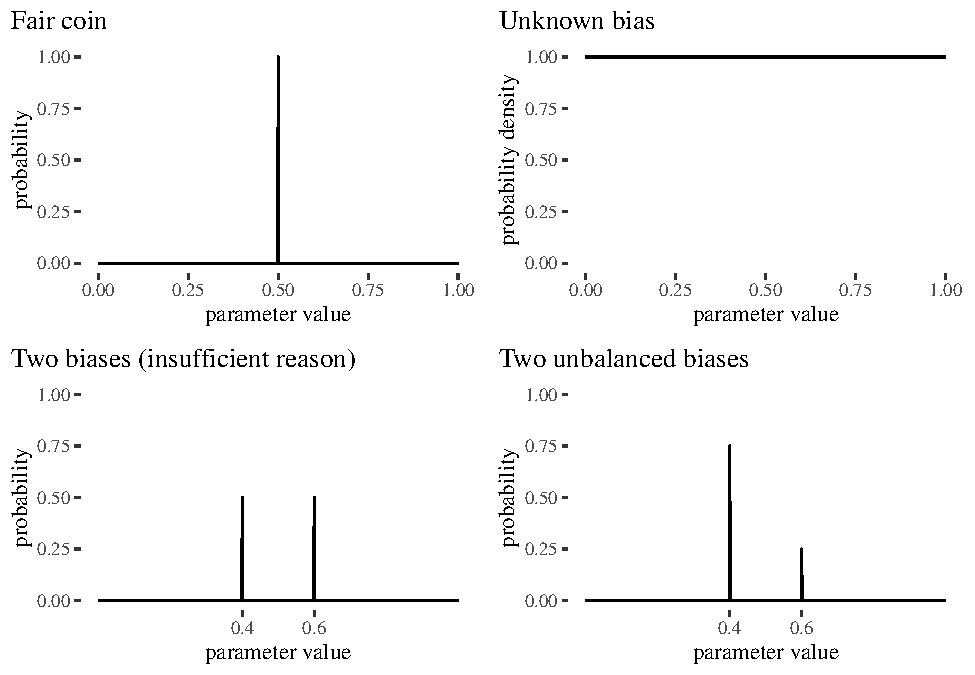
\includegraphics[width=0.8\linewidth]{imprecision_philosophical_paper2_files/figure-latex/FigevidenceResponse2-1} \end{center}
\caption{Examples of higher-order distributions for a few  scenarios problematic for both precise and imprecise probabilism.}
\label{fig:evidenceResponse}
\end{figure}

Besides its flexibility in modelling uncertainty, higher-order
probabilism does not fall prey to belief inertia. Consider a situation
in which you have no idea about the bias of a coin. So you start with a
uniform density over \([0,1]\) as your prior. By using binomial
probabilities as likelihoods, observing any non-zero number of heads
will exclude 0 and observing any non-zero number of tails will exclude 1
from the basis of the posterior. The posterior distribution will become
more centered around the parameter estimate as the observations come in.

Figure \ref{fig:intertia2} shows---starting with a uniform prior
distribution--- how the posterior distribution changes after successive
observations of heads, heads again, and then tails.\footnote{More
  generally, learning about frequencies, assuming independence and
  constant probability for all the observations, is modeled the Bayes
  way. You start with some prior density \(p\) over the parameter
  values. If you start with complete lack of information, \(p\) should
  be uniform. Then, you observe the data \(D\) which is the number of
  successes \(s\) in a certain number of observations \(n\). For each
  particular possible value \(\theta\) of the parameter, the probability
  of \(D\) conditional on \(\theta\) follows the binomial distribution.
  The probability of \(D\) is obtained by integration. That is:
  \begin{align*}
  p(\theta \vert D) & = \frac{p(D\vert \theta)p(\theta)}{p(D)}\\
  & = \frac{\theta^s (1-\theta)^{(n - s)}p(\theta)}{\int (\theta')^s (1-\theta')^{(n - s)}p(\theta')\,\, d\theta'}.
  \end{align*}} A further advantage of high-order probabilism over
imprecise probabilism is that the prospects for accuracy-based arguments
are not foreclosed. This is a significant shortcoming of imprecise
probabilism, especially because such arguments exist for precise
probabilism. One can show that there exist proper scoring rules for
higher-order probabilism. These rules can then be used to formulate
accuracy-based arguments. Another interesting feature of the framework
is that the point made by Schoenfield against imprecise probabilism does
not apply: there are cases in which accuracy considerations recommend an
imprecise stance (that is, a multi-modal distribution) over a precise
one. We will get back to these issues when we talk about accuracy.
\todo{Ref to section}

\begin{figure}

\begin{center}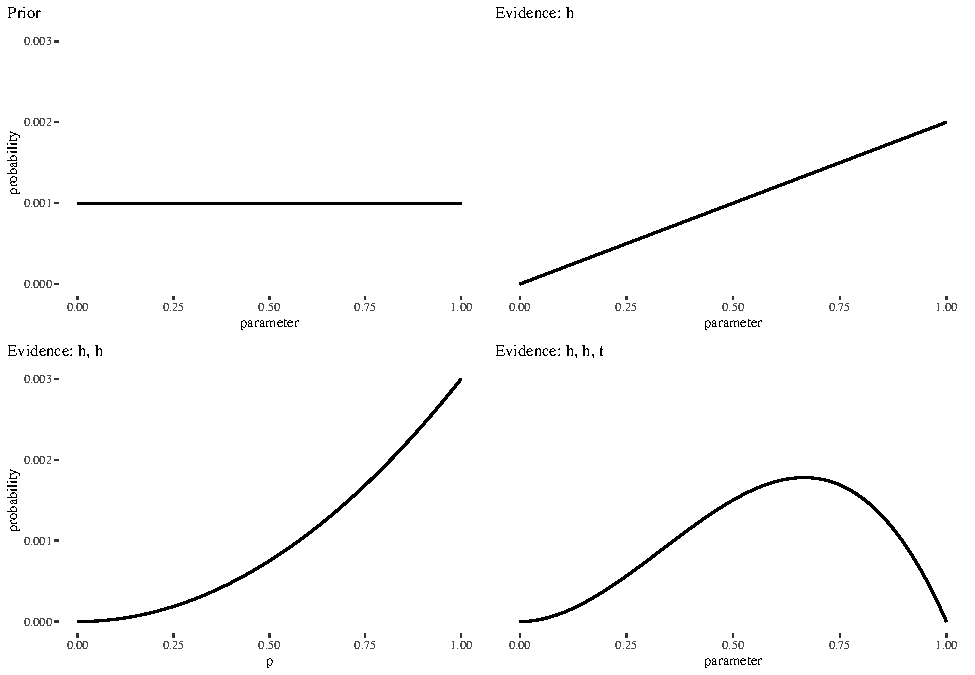
\includegraphics[width=0.8\linewidth]{imprecision_philosophical_paper2_files/figure-latex/Figinertia3-1} \end{center}
\caption{As observations of heads, heads and tails come in, extreme parameter values drop out of the picture and the posterior is shaped by the evidence.}
\label{fig:intertia2}
\end{figure}

\todo{The next two passages are somewhat new  and need to be carefully read and revised.}

The reader might be worried. The examples we discussed so far involve
estimation of chances or population frequencies; but how are we to
conceptualize higher order probabilities in a more general settings when
we think of first-order probabilities as RAs degrees of belief? One
might argue: since first-order probabilities capture one's uncertainty
about a proposition of interest, second-order probabilities are supposed
to capture one's uncertainty about how uncertain you are. But seems that
agents with a decent amount of introspection should be aware of how
uncertain they are, so ``estimating'' their first-order uncertainties
seems unnecessary.

Let us propose a somewhat more general picture that we hope will address
this concern. In many contexts, evidence justifies first-order
probability assignments (for instance, population frequency estimates)
to various degrees. For instance, suppose there is no evidence about the
bias of a coin. Then, each first-order point uncertainty about it would
be equally (un)-justified. If, instead, we know the coin is fair, the
evidence clearly selects one preferred value, .5. But often and with
respect to propositions other than straightforward propositions about a
frequency, evidence is stronger than the former case and weaker than the
latter case. The evidence justifies different values of first-order
uncertainty to various degrees. On our picture, second order
probabilities can be conceptualized in such a context as densities
capturing the extent to which different first-order uncertainties are
supported by the evidence.

Now, let's see how thinking in terms of higher-order probabilities can
be helpful in problems that are more realistic than coin tossing.

\hypertarget{a-more-concrete-example}{%
\section{A more concrete example}\label{a-more-concrete-example}}

In this section, we go over a stylized, but fairly realistic case in
which it makes an important difference whether we approach the problem
from the precise, imprecise, or higher-order perspective. A defendant in
a criminal case may face multiple items of incriminating evidence whose
strength can at least sometimes be assessed using probabilities. For
example, consider a murder case in which the police recover trace
evidence that matches the defendant. Hair found at the crime scene
matches the defendant's hair (call this evidence \textsf{hair}). In
addition, the defendant owns a dog whose fur matches the dog fur found
in a carpet wrapped around one of the bodies (call this evidence
\textsf{dog}).\footnote{The hair evidence and the dog fur evidence are
  stylized after two items of evidence in the notorious 1981 Wayne
  Williams case (Deadman, 1984b, 1984a).} The two matches suggest that
the defendant (and the defendant's dog) must be the source of the crime
traces (call this hypothesis \(\mathsf{source}\)). But how strong is
this evidence, really? What are the fact-finders to make of it?

The standard story among legal probabilists goes something like this
(Urbaniak \& Di Bello, 2021). To evaluate the strength of the two items
of match evidence, we must find the value of the likelihood ratio:
\[\frac{\pr{\s{dog}\wedge \s{hair} \vert \s{source}}}{\pr{\s{dog}\wedge \s{hair} \vert \neg \s{source}}}\]
For simplicity, the numerator can be equated to one. To fill in the
denominator, an expert provides the relevant random match probabilities.
Suppose the expert testifies that the probability of a random person's
hair matching the reference sample is about 0.0253, and the probability
of a random dog's hair matching the reference sample happens to be about
the same, 0.0256.\footnote{Probabilities have been slightly but not
  unrealistically modified to be closer to each other in order to make a
  conceptual point. The original probabilities were 1/100 for the dog
  fur, and 29/1148 for Wayne Williams' hair. We modified the actual
  reported probabilities slightly to emphasize the point that we will
  elaborate further on: the same first-order probabilities, even when
  they sound precise, may come with different degrees of second-order
  uncertainty.}

Presumably, the two matches are independent lines of evidence. In other
words, their random match probabilities must be independent of each
other conditional on either possible truth value of the source
hypothesis.\footnote{It is possible for \(A\) and \(B\) to be
  independent conditional on \(C\), but not conditional on \(\neg C\).
  Here, we require both independencies to hold.} Then, to evaluate the
overall impact of the evidence on the source hypothesis, you calculate:
\begin{align*}
\pr{\s{dog}\wedge \s{hair} \vert \neg \s{source}} & = \pr{\s{dog} \vert \neg \s{source}} 
\times \pr{\s{hair} \vert \neg \s{source}} \\
& =  0.0252613 \times  0.025641 = \ensuremath{6.4772626\times 10^{-4}}
\end{align*} This is a very low number. Two such random matches would be
quite a coincidence. The expert facilitates your understanding of how
this low number should be interpreted: they show you how the items of
match evidence change the probability of the source hypothesis given a
range of possible priors (Figure \ref{fig:impactOfPoint}). The posterior
of .99 is reached as soon as the prior is higher than 0.061.\footnote{These
  calculations assume that the probability of a match if the suspect and
  the suspect's dog are the sources is one.} While perhaps not
sufficient for outright belief in the source hypothesis, the evidence
seems extremely strong: a minor additional piece of evidence could make
the case against the defendant overwhelming.

\begin{figure}[H]

\begin{center}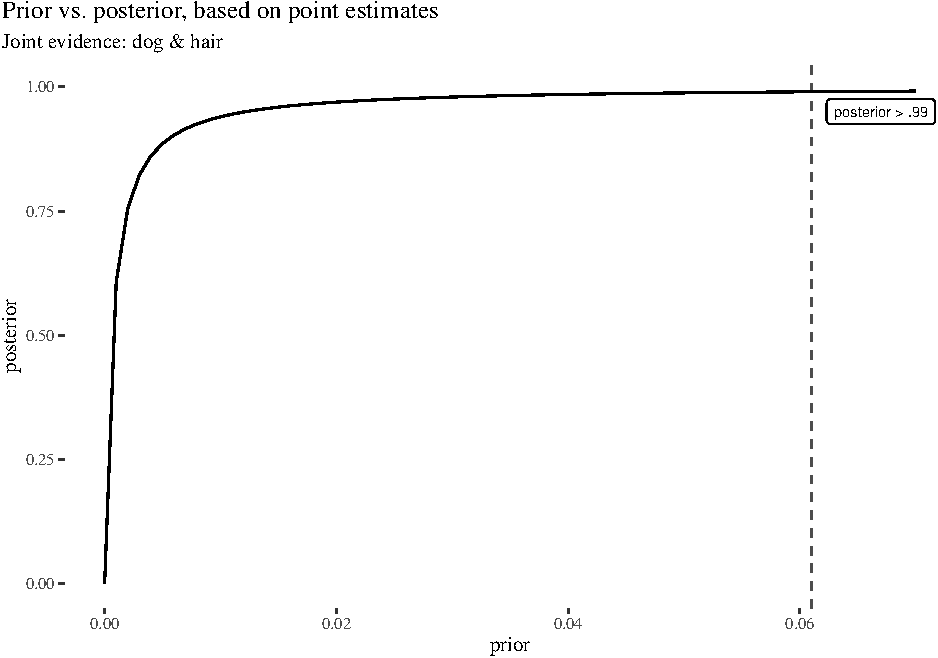
\includegraphics[width=0.6\linewidth]{imprecision_philosophical_paper2_files/figure-latex/impactOfPoint4-1} \end{center}
\caption{Impact of dog fur and human hair evidence on the prior, point estimates.}
\label{fig:impactOfPoint}
\end{figure}

Unfortunately, this analysis leaves out something crucial. You reflect
on what you have been told and ask the expert: how can you know the
random match probabilities with such precision? Shouldn't we also be
mindful of the uncertainty that may affect these numbers? The expert
agrees, and tells you that in fact the random match probability for the
hair evidence is based on 29 matches found in a database of size 1148,
while the random match probability for the dog evidence is based on
finding two matches in a reference database of size 78.

The expert's answer makes apparent that the precise random match
probabilities do not tell the whole story. Perhaps, the information
about sample sizes is good enough and now you know how to use the
evidence properly.\footnote{This is what, effectively, Taroni et al.
  (2015) seem to suggest when they insist the fact-finders should be
  simply given point estimates and information about the study set-up,
  such as sample size. We disagree.} But if you are like most human
beings, you can't. What to do, then?

You ask the expert for guidance: what are reasonable ranges of the
random match probabilities? What are the worst-case and best-case
scenarios? The expert responds with 99\% credible
intervals---specifically, starting with uniform priors, the ranges of
the random match probabilities are (.015,.037) for hair evidence and
(.002, .103) for fur evidence.\footnote{Roughly, the 99\% credible
  interval is the narrowest interval to which the expert thinks the true
  parameter belongs with probability .99. For a discussion of what
  credible intervals are, how they differ from confidence intervals, and
  why confidence intervals should not be used, see Kruschke (2015).}
With this information, you redo your calculations using the upper bounds
of the two intervals: \(.037\) and \(.103\). The rationale for choosing
the upper bounds is that these numbers result in random match
probabilities that are most favorable to the defendant. Your new
calculation yields the following: \begin{align*}
\mathsf{P}(\s{dog}\wedge \s{hair} \vert \neg \s{source})   & =  .037 \times .103 =.003811.
\end{align*} This number is around 5.88 times greater than the original
estimate. Now the prior probability of the source hypothesis needs to be
higher than 0.274 for the posterior probability to be above .99 (Figure
\ref{fig:impactOfCharitable}). So you are no longer convinced that the
two items of match evidence are strongly incriminating.

\begin{figure}[H]

\begin{center}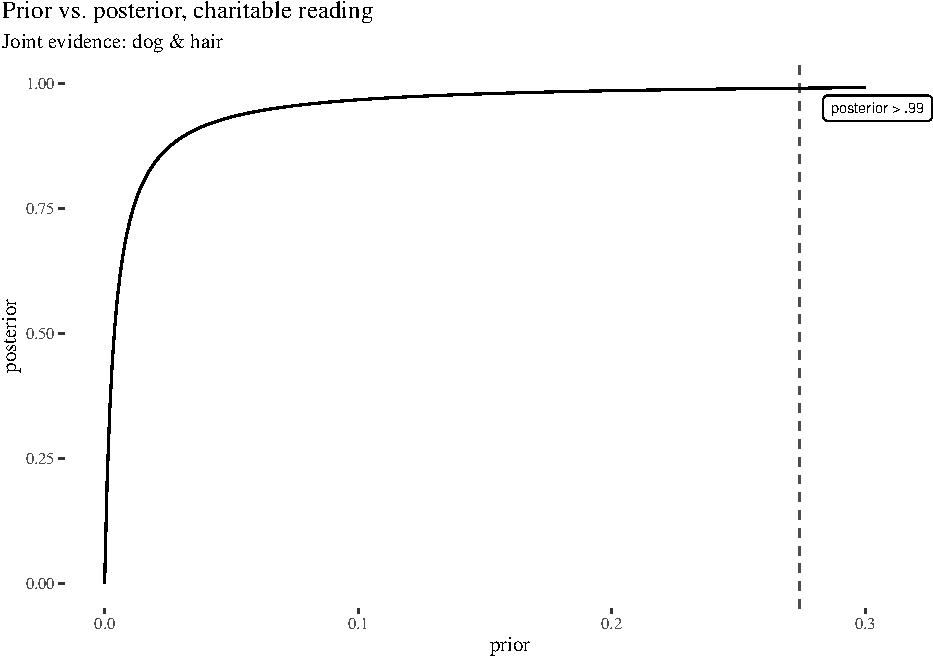
\includegraphics[width=0.6\linewidth]{imprecision_philosophical_paper2_files/figure-latex/FigcharitableImpact75-1} \end{center}

\caption{Impact of dog fur and human hair evidence on the prior, charitable reading.}
\label{fig:impactOfCharitable}
\end{figure}

This result is puzzling. Are the two items of match evidence strongly
incriminating evidence (as you initially thought) or somewhat weaker (as
the new calculation suggests)? For one thing, using precise random match
probabilities might be too unfavorable toward the defendant. On the
other hand, your new assessment of the evidence based on the upper
bounds might be too \emph{favorable} toward them. Is there a middle way
that avoids overestimating and underestimating the strength of the
evidence?

To see what this middle path looks like, we should reconsider the
calculations you just did. You made an important blunder: you assumed
that because the worst-case probability for one event is \(x\) and the
worst-case probability for another independent event is \(y\), the
worst-case probability for their conjunction is \(xy\). But this
conclusion does not follow if the margin of error (credible interval) is
fixed. The intuitive reason is simple: just because the probability of
an extreme (or larger absolute) value \(x\) for one variable \(X\) is
.01, and so it is for the value \(y\) of another independent variable
\(Y\), it does not follow that the probability that those two
independent variables take values \(x\) and \(y\) simultaneously is the
same. This probability is actually much smaller. The interval
presentation instead of doing us good led us into error.

In general, it is impossible to calculate the credible interval for the
joint distribution based solely on the individual credible intervals
corresponding to the individual events. We need additional information:
the distributions that were used to calculate the intervals for the
probabilities of the individual events. In our example, if you
additionally knew, for instance, that the expert used beta distributions
(as, arguably, they should in this context), you could in principle
calculate the 99\% credible interval for the joint distribution. It
usually will not be the same as whatever the results of multiplying the
individual interval edges, and it is unlikely that a human fact-finder
would be able to correctly run such calculations in their head even if
they knew the functional form of the distributions used.\footnote{Also,
  in principle, in more complex contexts, we need further information
  about how the items of evidence are related if we cannot take them to
  be independent.} So providing the fact-finder with individual
intervals, even if further information about the distributions is
provided, might easily mislead.\footnote{Investigation of the extent to
  which the individual interval presentation is misleading would be an
  interesting psychological study.}

As it turns out, given the reported sample sizes, the 99\% credible
interval for the probability
\(\mathsf{P}(\s{dog}\wedge \s{hair} \vert \neg \s{source})\) is
\((0.000023, 0.002760)\). The upper bound of this interval would then
require the prior probability of the source hypothesis to be above .215
for the posterior to be above .99. On this interpretation, the two items
of match evidence are still not quite as strong as you initially
thought, but stronger than what your second calculation indicated.

We still should think of credible intervals as rough summaries, which
might be useful if the underlying distributions are fairly symmetrical,
or narrow enough. But in our case, they might not be. For instance,
Figure \ref{Figdensities} depicts beta densities for dog fur and human
hair, together with sampling-approximated density for the joint
evidence.\\
The distribution for the joint evidence is not symmetric. If you were
only informed about the edges of the interval, you would be oblivious to
the fact that the most likely value (and the bulk of the distribution,
really) does not simply lie in the middle between the edges. Just
because the parameter lies in an interval with some posterior
probability, it does not mean that the ranges near the edges of the
interval are equally likely---the bulk of the density might very well be
closer to one of the edges. Therefore, only relying on the edges can
lead one to either overestimate or underestimate the probabilities at
play. This also means that---following our advice on how to illustrate
the impact of evidence on prior probabilities---a better representation
of the dependence of the posterior on the prior should comprise multiple
possible sampled lines whose density mirrors the density around the
probability of the evidence (Figure \ref{Figlines}).

\begin{figure}[H]

\begin{center}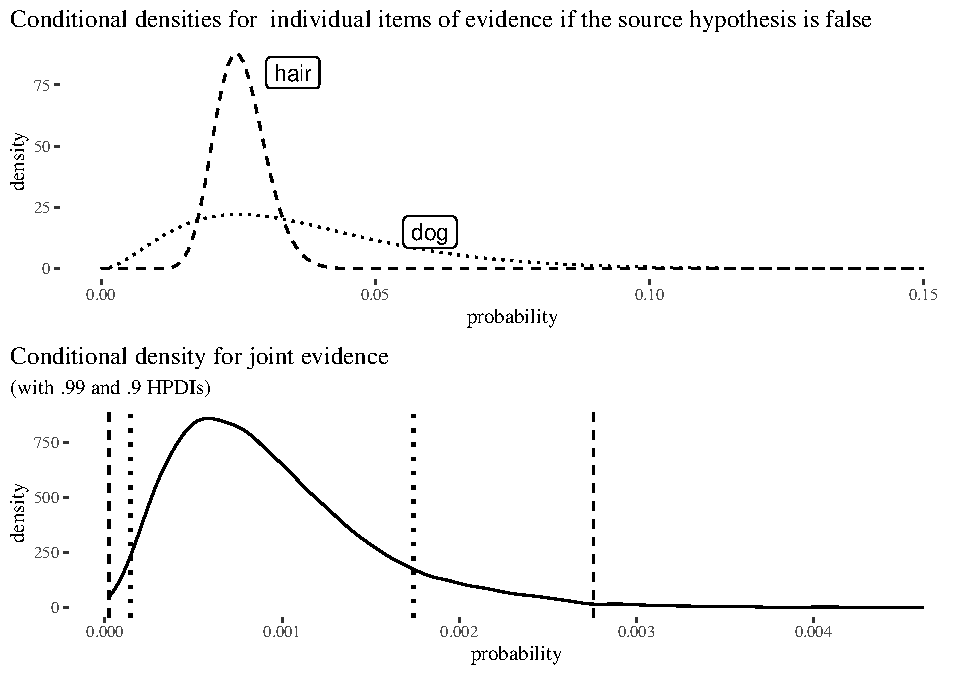
\includegraphics[width=0.8\linewidth]{imprecision_philosophical_paper2_files/figure-latex/Figdensities-1} \end{center}
\caption{Beta densities for individual items of evidence and the resulting joint density with .99 and .9 highest posterior density intervals, assuming the sample sizes as discussed and independence, with uniform priors.}
\label{Figdensities}
\end{figure}

\begin{figure}[H]

\begin{center}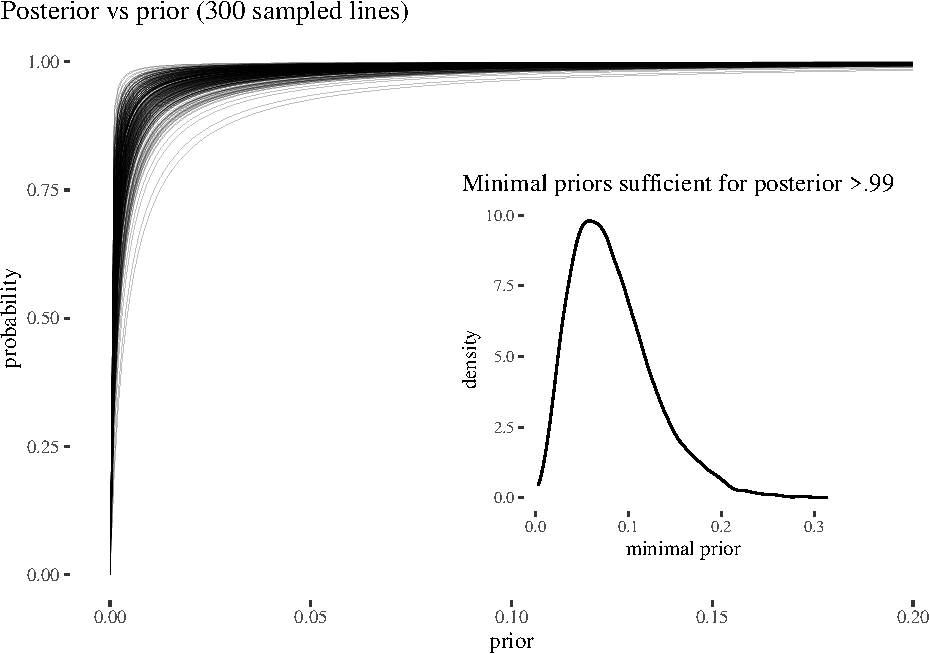
\includegraphics[width=0.85\linewidth]{imprecision_philosophical_paper2_files/figure-latex/Figlines5-1} \end{center}

\caption{300 lines illustrating the uncertainty about the dependence of the posterior on the prior given aleatory uncertainty about the evidence, with the distribution of the minimal priors required for the posterior to be above .99.}

\label{Figlines}

\end{figure}

This, then, is the main claim illustrated in this section: higher-order
approach to evidence evaluation is more reliable and more honest about
the uncertainties involved. Whenever density estimates for the
probabilities of interest are available (and they should be available
for match evidence and many other items of scientific evidence if the
reliability of a given type of evidence has been properly studied),
those densities should be reported for assessing the strength of the
evidence. This approach avoids hiding actual aleatory uncertainties
under the carpet. It also allows for a balanced assessment of the
evidence, whereas using point estimates or intervals may exaggerate or
underestimate the value of the evidence.

Mathematically, we do not propose anything radically new---we just put
together some of the items from the standard Bayesian toolkit. The
novelty is rather in our arguing that that these tools are
under-appreciated in formal epistemology and in the legal scholarship
and should be properly used to incorporate second-order uncertainties in
evidence evaluation and incorporation.

--\textgreater{}

\hypertarget{computational-and-representational-considerations}{%
\section{Computational and representational
considerations}\label{computational-and-representational-considerations}}

The higher-order framework we are advocating is not only applicable to
the evaluation of individual pieces of evidence. Complex bodies of
evidence and hypotheses---for example, those often represented by
Bayesian networks---can also be approached from this perspective. The
general strategy is this: (1) capture the uncertainties involving the
individual items of evidence in a modular fashion using the standard
tools for statistical inference. (2) Elicit other probabilities or
densities from experts\footnote{For expert elicitation of densities in a
  parametric fashion and the discussion of the improvement to which
  doing so instead of eliciting point values leads, see (O'Hagan et al.,
  2006).}, (3) put those together using a structure similar to that of a
Bayesian network, except allowing for uncertainties of various levels to
be put together --- a usual tool for such a representation is a
probabilistic program (Bingham et al., 2021), and (4) perform inference
evaluating the relevant probabilities or densities of interest.

If the reader is more used to thinking in terms of Bayesian networks, a
somewhat restrictive but fairly straightforward way to conceptualize a
large class of such programs is to imagine a probabilistic program as
stochastically generating Bayesian networks using our uncertainty about
the parameter values, update with the evidence, and propagate
uncertainty to approximate the marginal posterior for nodes of interest.

As an illustration, let us start with a simplified Bayesian network
developed by Fenton \& Neil (2018). The network is reproduced in Figure
\ref{fig:scBNplot} and represents the key items of evidence in the
infamous British case R. v. Clark (EWCA Crim 54, 2000).\footnote{Sally
  Clark's first son died in 1996 soon after birth, and her second son
  died in similar circumstances a few years later in 1998. At trial, the
  pediatrician Roy Meadow testified that the probability that a child
  from such a family would die of Sudden Infant Death Syndrome (SIDS)
  was 1 in 8,543. Meadow calculated that therefore the probability of
  both children dying of SIDS was approximately 1 in 73 million. Sally
  Clark was convicted of murdering her infant sons. The conviction was
  reversed on appeal. The case of appeal was based on new evidence:
  signs of a potentially lethal disease were found in one of the bodies.}

In a Bayesian network the arrows depict direct relationships of
influence between variables, and nodes---conditional on their
parents---are taken to be independent of their non-descendants.
\textsf{Amurder} and \textsf{Bmurder} are binary nodes corresponding to
whether Sally Clark's sons, call them A and B, were murdered. These
nodes influence whether signs of disease (\textsf{Adisease} and
\textsf{Bdisease}) and bruising (\textsf{Abruising} and
\textsf{Bbruising}) were present. Also, since A's death preceded in time
B's death, whether A was murdered casts some light on the probability
that B was also murdered.

The choice of the probabilities in the network is quite specific, and it
is not clear where such precise values come from. The standard response
invokes \emph{sensitivity analysis}: a range of plausible values is
tested. As already discussed, this approach ignores the shape of the
underlying distributions. Sensitivity analysis does not make any
difference between probability measures (or point estimates) in terms of
their plausibility, but some will be more plausible than others.
Moreover, if the sensitivity analysis is guided by extreme values, these
might play an undeservedly strong role. These concerns can be addressed,
at least in part, by recourse to higher-order probabilities. In a
precise Bayesian network, each node is associated with a probability
table determined by a finite list of numbers (precise probabilities).
But suppose that, instead of precise numbers, we have densities over
parameter values for the numbers in the probability tables.\footnote{The
  densities of interests can then be approximated by (1) sampling
  parameter values from the specified distributions, (2) plugging them
  into the construction of the BN, and (3) evaluating the probability of
  interest in that precise BN. The list of the probabilities thus
  obtained will approximate the density of interest. In what follows we
  will work with sample sizes of 10k.} An example for the Sally Clark
case is represented in Figure \ref{fig:SCwithHOP}.

\begin{figure}[H]

\begin{center}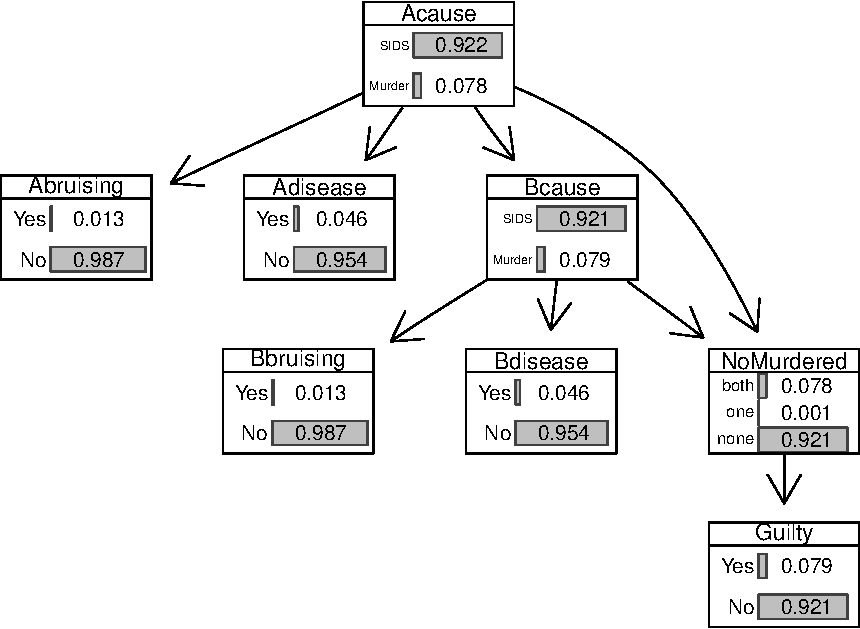
\includegraphics[width=0.5\linewidth]{imprecision_philosophical_paper2_files/figure-latex/scBNplot2-1} \end{center}
\caption{Bayesian network for the Sally Clark case, with marginal prior probabilities.}
\label{fig:scBNplot}
\end{figure}

\begin{figure}[H]

\begin{center}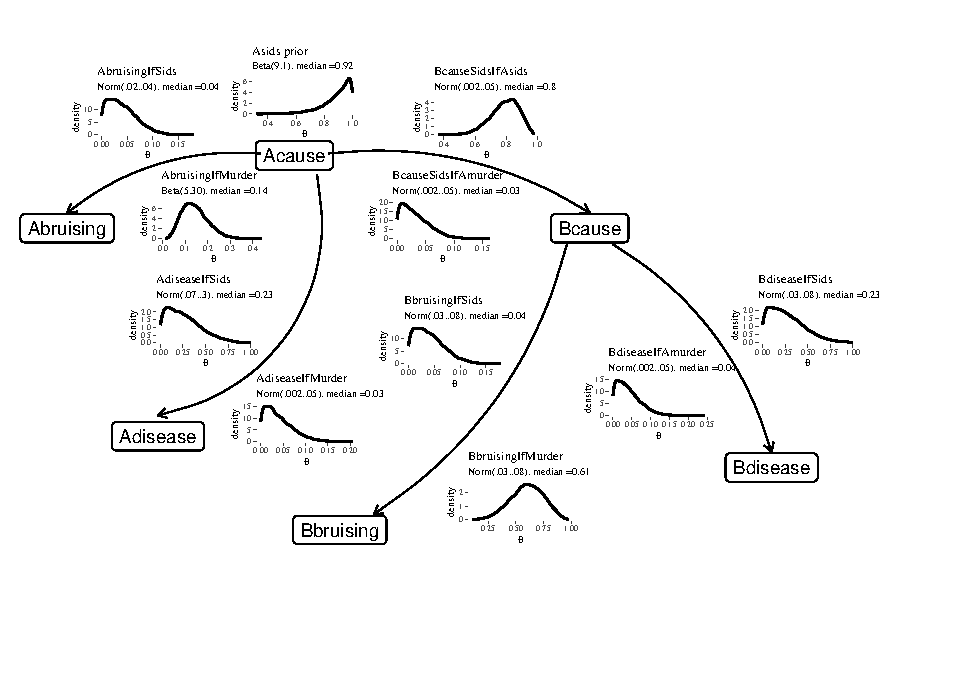
\includegraphics[width=1.1\linewidth,height=2\textheight,angle=90]{imprecision_philosophical_paper2_files/figure-latex/SCwithHOP-1} \end{center}

\caption{An illustration of a probabilistic program for the Sally Clark case.}
\label{fig:SCwithHOP}
\end{figure}

Using the probabilistic program, we can investigate the impact of
different items of evidence on Sally Clark's probability of guilt
(Figure \ref{fig:SCwithHOP2}). The starting point is the prior density
for the \s{Guilt} node (first graph). Next, the network is updated with
evidence showing signs of bruising on both children (second graph).
Next, the assumption that both children lack signs of potentially lethal
disease is added (third graph). Finally, we consider the state of the
evidence at the time of the appellate case: signs of bruising existed on
both children, but signs of lethal disease were discovered only on the
first child. Interestingly, in the strongest scenario against Sally
Clark (third graph), the median of the posterior distribution is above
.95, but the uncertainty around that median is still too wide to warrant
a conviction.\footnote{The lower limit of the 89\% Highest Posterior
  Density Intervals (HPDI) is at .83.} This underscores the fact that
relying on point estimates can lead to overconfidence. Paying attention
to the higher-order uncertainty about the first-order probability can
make a difference to trial decisions.

\begin{figure}[H]

\begin{center}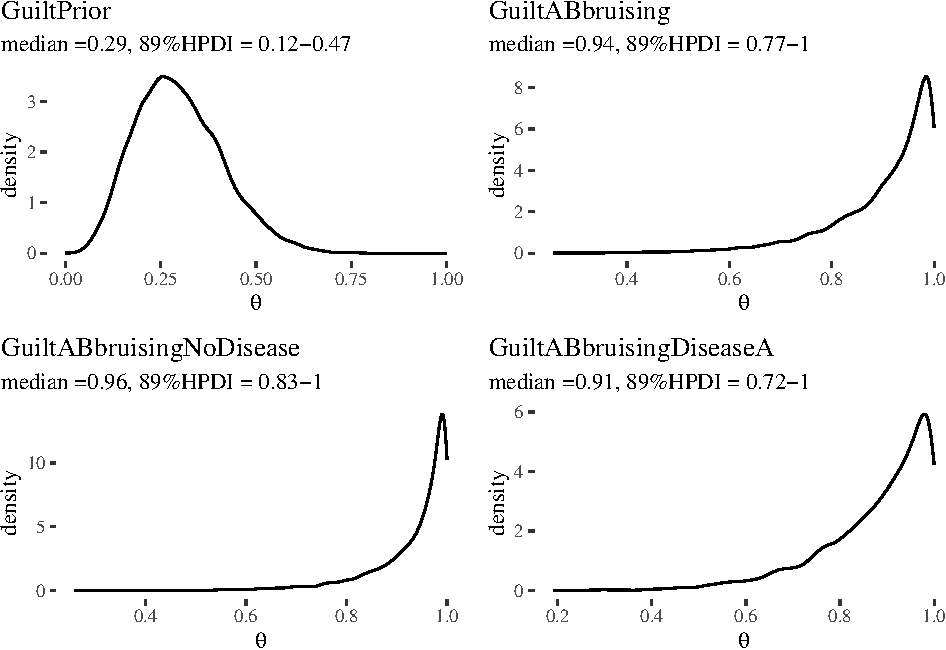
\includegraphics[width=0.9\linewidth]{imprecision_philosophical_paper2_files/figure-latex/SCwithHOP2-1} \end{center}


\caption{Impact of incoming evidence in the Sally Clark case.}
\label{fig:SCwithHOP2}
\end{figure}

One question that arises is how this approach relates to the standard
method of using likelihood ratios to report the value of the evidence.
On this approach, the conditional probabilities that are used in the
likelihood ratio calculations are estimated and come in a package with
an uncertainty about them. Accordingly, these uncertainties propagate:
to estimate the likelihood ratio while keeping track of the uncertainty
involved, we can sample probabilities from the selected distributions
appropriate for the conditional probabilities needed for the
calculations, then divide the corresponding samples, obtaining a sample
of likelihood ratios, thus approximating the density capturing the
recommended uncertainty about the likelihood ratio. Uncertainty about
likelihood ratio is just propagated uncertainty about the involved
conditional probabilities. For instance, we can use this tool to gauge
our uncertainty about the likelihood ratios corresponding to the signs
of bruising in son A and the presence of the symptoms of a potentially
lethal disease in son A (Figure \ref{fig:SClrs}).

\begin{figure}[H]


\begin{center}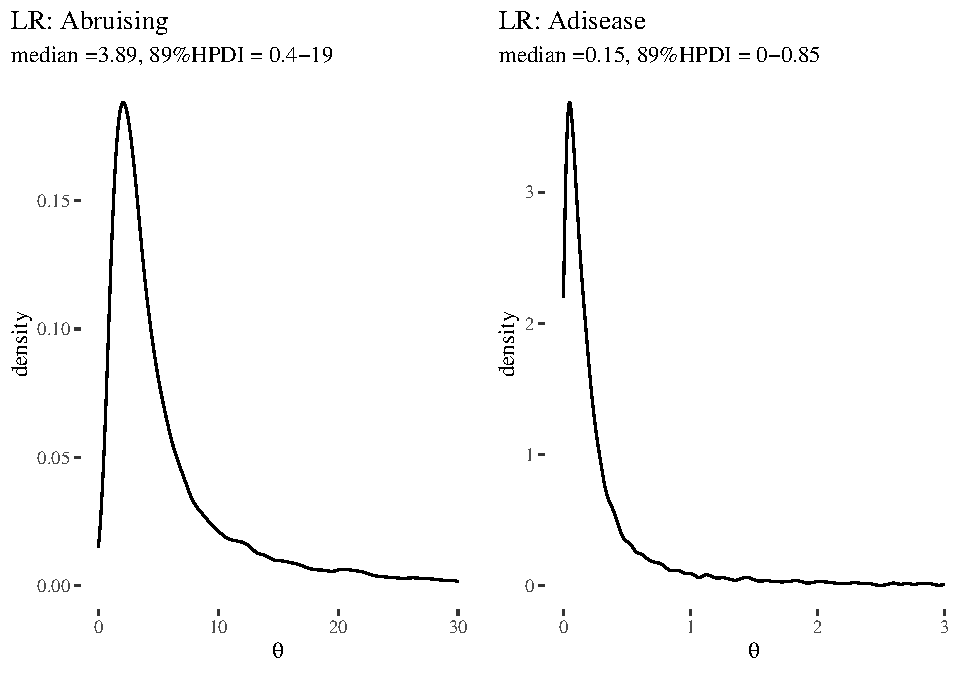
\includegraphics[width=0.9\linewidth]{imprecision_philosophical_paper2_files/figure-latex/SClrs-1} \end{center}

\caption{Likelihood ratios forbruising and signs of disease in child A in the Sally Clark case.}
\label{fig:SClrs}

\end{figure}

\hypertarget{accuracy-in-the-second-order-setting}{%
\section{Accuracy in the second-order
setting}\label{accuracy-in-the-second-order-setting}}

\hypertarget{accuracy}{%
\subsection{Accuracy}\label{accuracy}}

As we already discussed, one challenge for the imprecisers is providing
a workable scoring rule that would be a counterpart of, say, the Brier
scoring rule for the precise case. While the imprecisers have hard time
defining what the accuracy of a set of measures is, our path is easier.
Already some work has been done on the notion of accuracy of continuous
probability distributions (Hersbach (2000), Pettigrew (2012), Gneiting
\& Raftery (2007)). One key notion in use is that of continuous ranked
probability score (CRPS) of a distribution \(p\) with respect to a
possible world \(w\): \begin{align*}
I(p,w) &= \int_{-\infty}^\infty \vert \mathsf{P}(x) - \mathbf{ 1 }(x\geq V(w))\vert ^2 \, dx
\end{align*} \noindent where \(\mathsf{P}\) is the cumulative
probability corresponding to a given density, and \begin{align*}
\mathbf{ 1 }(x \geq V(w)) & = \begin{cases} 1 & \text{ if } x \geq V(w)\\
0 & \text{ o$\,$/w. }
\end{cases}
\end{align*} \noindent  The intuition here is that the measure takes the
Cramer-Von-Mises measure of distance between densities, defined in terms
of the area under the squared euclidean distances between the
corresponding cumulative density functions: \begin{align*}
\mathcal{C}(p,q) & = \int_{0}^{1} \vert P(x) - Q(x)\vert^2 \, dx
\end{align*} \noindent and uses it to measure distance to an
epistemically omniscient chance hypothesis, which either puts full
weight on 0, if a given proposition is false, or on 1, otherwise. We
will start building by reflecting on this approach.

First, as in practice we are unable to work with infinite precision
anyway, not much harm is done and much computational ease is made with
(grid) approximations, so we will keep using these in line with the
previous developments (note for instance that there are no readily
computable solutions to the integral used in the definition of CRPS,
although it can sometimes be evaluated in closed form) (Gneiting \&
Raftery, 2007, p. 366). So, instead of integration, we'll be using
summation over the values for a finite number of bins.

Now, let's see how this approach would play out in a scenario very much
like Schoenfield's (EMC), with an additional layer of uncertainty: the
opponent will produce two coins, one with the distribution of Heads
either normal around \(.3\), and one normal around \(.5\), both with the
standard deviation of \(.05\), randomly pick one of these coins and then
toss it. The RA knows the setup. Consider the following three (out of
many) possible stances that RA could take:

\begin{figure}[H]

\begin{center}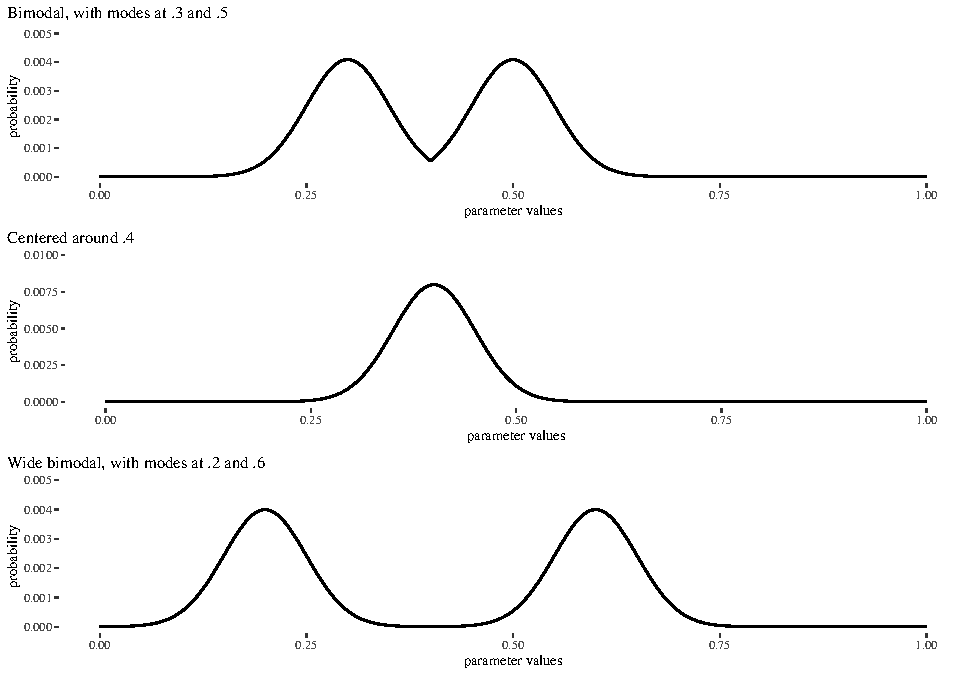
\includegraphics[width=1\linewidth]{imprecision_philosophical_paper2_files/figure-latex/figEMC-1} \end{center}
\caption{Three (out of many) candidates in a vague EMS scenario. All distributions are built from normal  distributions with standard deviation $.5$, the bimodal ones are "glued" in the middle.}
\label{fig:EMC}
\end{figure}

An impreciser might be inclined to say that it is the bimodal
distribution that's appropriately evidence-responsive. The centered one,
while centering on the expected value, definitely gets the chances
wrong, while the wide bimodal has its guesses too close to truth values
and too far from the actual known chances. Now, is this in any way
mirrored by CRPS and expected CRPS calculations? It turns out it isn't.

\begin{table}[H]
\centering
\begin{tabular}{lrrrrrr}
\toprule
distribution & CRPS1 & CRPS0 & KLD1 & KLD0 & ExpCRPS & ExpKLD\\
\midrule
bimodal & 534.7305 & 334.9305 & 80.06971 & 33.90347 & 414.8505 & 52.36997\\
centered & 571.2192 & 371.4192 & 110.84220 & 53.13440 & 451.3392 & 76.21752\\
wide bimodal & 485.4052 & 285.6177 & 54.13433 & 19.50965 & 365.5340 & 33.35974\\
\bottomrule
\end{tabular}
\caption{CPRS and KLD inaccuracies of the three distributions to the TRUE and FALSE omniscient functions, with expected inaccuracies.}
\end{table}

Notice that the expected inaccuracy recommend the wide bimodal
distribution, which does not seem desirable! This, notice also, doesn't
change if instead of CRPS we use the KL divergence from the omniscient
measure, so it doesn't seem like the choice of the measure itself is the
culprit here.

The problem here is that all these distributions have the same expected
value: \(.4\), which is used in the calculations of the expected
inaccuracies. This also means that not only the wide bimodal
distribution expects itself to be the least inaccurate, but also that
other measures expect it to be the least inaccurate! This also suggests
that the strategy of (i) calculating two distances/divergencies from the
two extreme omniscient measures and (ii) averaging by plugging in the
expected value, does not result in a proper inaccuracy score.

But this strategy is clearly against the spirit of our enterprise. If we
start with the idea that expected values are often not good
representations of RA's uncertainty, it is not terribly surprising that
they do not lead to sensible expected inaccuracy calculations. After
all, since the three distributions do have the same expected value, the
difference between the probabilities they assigned don't seem to be
taken seriously in the weighting stage (ii). The question now is, how
can we do justice to the complexity of RA's credal state in the expected
inaccuracy considerations?

Well, if we start with taking RA's higher order probabilities to be
probabilities about which parameter values are the right ones (true
chances, real population frequencies, the point credences justified by
the evidence, or what have you, philosophically speaking), we should see
how taking these intuitions seriously plays out. So, instead of
measuring inaccuracy with respect to two omniscient credences peaking at

either 0 or 1 and averaging using expected values, we should instead
look at \(n\) potential true probability hypotheses, each of them
pointed at a single bin in our approximation, calculate all the
inaccuracies with respect to their corresponding omniscient functions,
and calculate the expected inaccuracies scores using whole distributions
rather than their expected values.

For the three distributions we're discussing in this chapter, the
inaccuracies calculated using CRPS and KL divergence with respect to
various potential true probability distributions look as in Figure
\ref{fig:inaccuracies2}.

\begin{figure}[H]

\begin{center}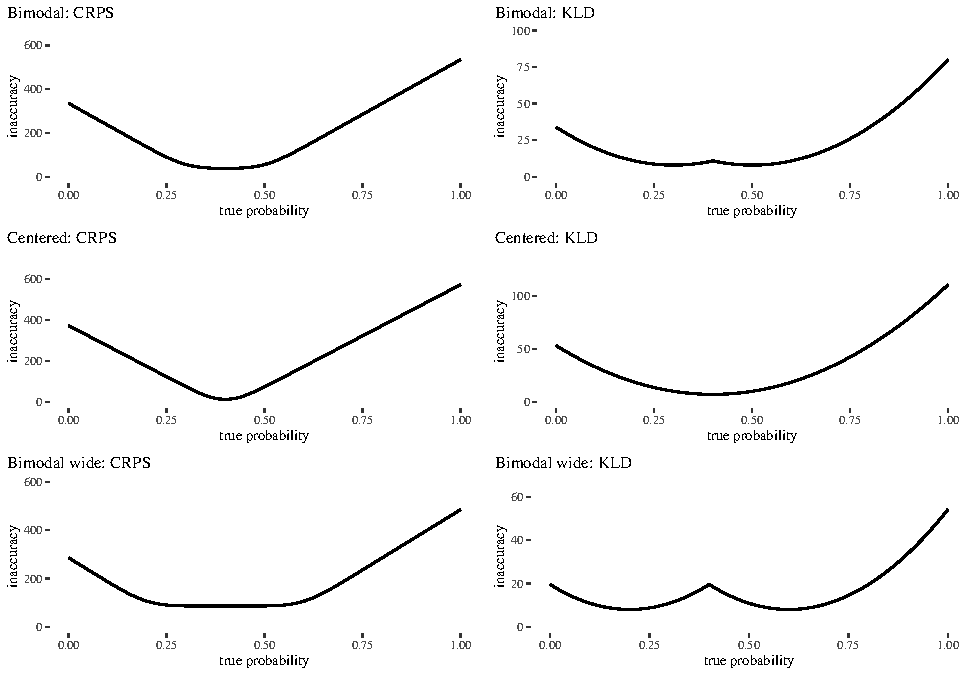
\includegraphics[width=1\linewidth]{imprecision_philosophical_paper2_files/figure-latex/figinaccuracies2-1} \end{center}


\caption{CLPSR and KL divergence based inaccuracies vs (omniscient functions corresponding to) $n$ true 
probability hypotheses for the three distributions discussed in this section.}
\label{fig:inaccuracies2}
\end{figure}

One important difference transpires between using CRPS rather than KLD.
Notice how for chance hypotheses between the actual peaks the inaccuracy
remains flat. This seems to be an artifice of choosing a squared
distance metric. If instead we go with a more principled,
information-theory-inspired KL divergence, inaccuracy in fact jumps a
bit for values in between the peaks for the bimodal distributions, which
seems intuitive and desirable.

Note that now the expected inaccuracies of the distributions from their
perspective look as in \mbox{Table \ref{tab:expected2}.}

\begin{table}[H]
\begin{tabular}{lrrrrrr}
& \multicolumn{3}{c}{CPRS} & \multicolumn{3}{c}{KLD} \\
\toprule
  & bimodal & centered & wide bimodal & bimodal & centered & wide bimodal\\
\midrule
bimodal & 64.670 & 78.145 & 88.380 & 8.577 & 10.655 & 11.336\\
centered & 41.657 & 28.181 & 85.911 & 9.239 & 7.690 & 15.627\\
wide bimodal & 137.699 & 171.719 & 113.989 & 11.541 & 19.231 & 8.689\\
\bottomrule
\end{tabular}
\caption{Expected inaccuracies of the three distributions from their own perspectives.
 Each row corresponds to a perspective.}
\label{tab:expected2}
\end{table}

Note that now the results are as intuitively they should: each
distribution recommends itself. How does the framework capture the idea
that it is the bimodal distribution that seems more adequate than the
others?

Well, one way to go would be to measure inaccuracy with respect to the
only chance hypotheses that should be on the table, given the
testimonial evidence. \(H_3\) on which the true chance is \(.3\) and
\(H_5\) on which the true chance is \(.5\). The respective inaccuracies
are as in Table \ref{tab:schoen}.

\begin{table}[H]
\begin{tabular}{lrrrr}
 & \multicolumn{2}{c}{CRPS} & \multicolumn{2}{c}{KLD} \\
\toprule
&H3 & H5 & H3 & H5\\
\midrule
bimodal &55.475 & 55.378 & 7.935 & 7.935\\
centered &72.281 & 72.090 & 9.836 & 9.825\\
wide bimodal & 86.230 & 86.223 & 10.871 & 10.882\\
\bottomrule
\end{tabular}
\caption{CRPS and KLD inacurracies of the three distributions with respect to the two hypotheses.
 Note that on both inaccuracy measures the bimodal distribution dominates the other two.}
\label{tab:schoen}
\end{table}

Just to double-check if some of this desirable outcome isn't caused by
not using pointed credences, we can run the calculations using the
pointy version: with all the weight on .4, or weights split in half,
either between \(.3\) and \(.5\), or between \(.2\) and \(.6\). As
expected, inaccuracy considerations recommend the bimodal version,
whichever of the two hypotheses holds (Table \ref{tab:schoen2}).

\begin{table}[H]
\begin{tabular}{lrrrr}
 & \multicolumn{2}{c}{CRPS} & \multicolumn{2}{c}{KLD} \\
\toprule
 &H3 & H5 & H3 & H5\\ \midrule
pointed bimodal &49.75 & 49.75 & 1.00 & 1.00\\
pointed centered &100.00 & 100.00 & 16.61 & 16.61\\
pointed wide bimodal & 99.75 & 99.75 & 16.61 & 16.61\\
\bottomrule
\end{tabular}
\caption{CRPS and KLD inacurracies of the three pointed distributions with respect to the two hypotheses.}
\label{tab:schoen2}
\end{table}

Now, the reader might worry that this has been only a discussion of an
example, which fails to establish the strict propriety of the KLD
inaccuracy measure. Fair point. In fact, such a proof is given in the
appendix to this paper. Just to get the gist of the argument, consider
taking the inaccuracy of a second-order discretized probability mass
\(p\) over a parameter space \([0,1]\), given that the real probability
is \(\theta\) as the Kullback-Leibler divergence of \(p\) from the
indicator distribution of \(\theta\) (which assigns 1 to \(\theta\) and
0 to all other parameter values in the parameter space), denoted as
\(\mathcal{I}_{\dkl}^2\).\footnote{The argument generalizes to parameter
  spaces that correspond to probabilities of multiple propositions which
  are Cartesian products of parameter spaces explicitly used in the
  argument in this section.} It turns out that this is a strictly proper
inaccuracy measure: each \(p\) expects itself to be the least inaccurate
distribution. The argument has four key moves.

\begin{enumerate}
\item the inaccuracy of $p$ w.r.t. to parameter $\theta$ is just $- \log_2 p(\theta)$,
\item  the expected inaccuracy of $p$ from the perspective of $p$ is the entropy of $p$, $H(p)$,
\item  the inaccuracy of $q$ from the perspective of $p$ is the cross-entropy $H(p,q)$,
\item and it is an established result that cross-entropy is strictly larger than entropy as soon as $p\neq q$.
  \end{enumerate}

\hypertarget{discussion}{%
\section{Discussion}\label{discussion}}

Our approach does involve multiple parameters, uncertainty about them,
along with a dependency structure between random variables. So it is
only natural to ask whether what we propose is not just an old wolf in a
new sheep's clothing, as one might think that what looks like a DAG and
quacks like a DAG is always a hierarchical model. In this section we
briefly clarify what the answer to this question is.

First, we need some clarity on what a Bayesian hierarchical model is. In
the widest sense of the word, these are mathematical descriptions
involving multiple parameters such that credible values for some of them
meaningfully depend on the values of other parameters, and that
dependencies can be re-factored into a chain of dependencies. For
instance, think about a joint parameter space for two parameters
\(\theta\) and \(\omega\), where
\(p(\theta, \omega \vert D) \propto p(D \vert \theta, \omega)p(\theta, \omega)\).
If, further, some independence-motivated re-factoring of the right-hand
side---for instance as
\(p(D\vert \theta)p(\theta \omega)p(\omega)\)---is possible, we are
dealing with a hierarchical model in the wide sense of the word.

Such models usually come useful when we are dealing with clustered data,
such as a cohort study with repeated measures, or some natural groupings
at different levels of analysis. Then, lower-level parameters are
treated as i.i.d. and share the same parameter distribution
characterized by some hyper-parameters in turn characterized by a prior
distribution. As a simple example consider a scenario in which we are
dealing with multiple coins created by one mint---each coin has its own
bias \(\theta_i\), but also there is some commonality as to what these
biases are in this mint, represented by a higher-level parameter
\(\theta\). Continuing the example, assume
\(\theta_i \sim \mathsf{Beta}(a, b)\) and
\(y_{i\vert s} \sim \mathsf{Bern}(\theta_s)\), where the former
distribution can be re-parametrized as
\(\mathsf{Beta}(\omega(k-2)+1, (1-\omega)(k-2)+1)\). Let's keep \(k\)
fixed, \(\omega\) is our expected value of the \(\theta_i\) parameters,
with some dispersion around it determined by \(k\). Now, if we also are
uncertain about \(\omega\) and express our uncertainty about it in terms
a density \(p(\omega)\), we got ourselves a hierarchical model with
joint prior distribution over parameters
\(\prod p(\theta_i \vert \omega) p(\omega)\).

As another example, one can develop a multilevel regression model of the
distributions of the random levels in various counties, where both the
intercept and the slope vary with counties by taking\\
\(y_i\sim \mathsf{Norm}(\alpha_{\mbox{j[i]}}\, + \beta_{\mbox{j[i]}} x_i, \sigma^2_y )\),
where \(j\) is a county index,
\(\alpha_j \sim \mathsf{Norm}(\mu_\alpha,\sigma_\alpha^2 )\), and
\(\beta_j \sim \mathsf{No}rm(\mu_\beta,\sigma_\beta^2 )\). Then, running
the regression one estimates both the county-level coefficients, and the
higher-level parameters.

Our approach is similar to the standard hierarchical models in the most
general sense:\\
there is a meaningful independence structure and distributions over
parameter values that we are working with. However, our approach is
unlike such models in a few respects. For one, we are not dealing with
clustered data, and the random variables are mostly propositions and
their truth values. Given a hypothesis \(H\) and an item of evidence
\(E\) for it, there seems to be no interesting conceptualization on
which the underlying data would be clustered. For example, considering
stains at a crime scene as a subgroup of crimes being committed doesn't
make logical sense. Yes, there is dependency between these phenomena,
but describing it as clustering would be at least misleading. Second,
the dependencies proceed through the values of the random variables
which are \textbf{not} parameters, but rather truth-values, and require
also conditional uncertainties regarding the dependencies between these
truth-values.

Again, continuing the hypothesis-evidence example, we have
\(H \sim \mathsf{Bern}(p_h)\), \(p_h \sim \mathsf{Beta}(a_h, b_h)\), and
\(E\sim \mathsf{Bern}(p_e)\). But then we also have the beta
distributions for the probability of the evidence conditional on the
actual values of the random variables---the truth-values---thus
\(p_e \vert H = 1 \sim beta(a_{+}, b_{+} )\) and
\(p_e \vert H = 0 \sim \mathsf{Beta}(a_{-}, b_{-})\). But the
re-factoring in terms of the actual values of the random variables
(which just happen to resemble probabilities because they are truth
values) makes it quite specific, at the same time allowing for the
computational use of a probabilistic program. Finally, the reasoning we
describe is not a regression the way it is normally performed: the
learning task is delegated to the bottom level of whatever happens to
the Bayesian networks once updated with evidence. We would prefer to
reserve the term \emph{hierarchical model} for a class of models dealing
with interesting cluster structures in the data. A more fitting term for
the representation tool we propose should be used here is
\emph{probabilistic programs}. We do not claim any originality in
devising this tool: it's an already existing tool. What we argue for,
though, is its ability for being usefully deployed in the context of
forensic evidence evaluation and integration with other assumptions and
hypotheses.

Perhaps, you might dislike the idea of going higher-order for
theoretical reasons. One might be that you don't like the complexity.
This seems to be the line taken by Bradley, who refuses to go
higher-order for the following reason:

\begin{quote}
Why is sets of probabilities the right level to stop the regress at? Why not sets of sets? Why not second-order 
probabilities? Why not single probability functions? This is something of a pragmatic choice. The further we 
allow this regress to continue, the harder it is to deal with these belief representing objects. So let's not
 go further than we need. 131-132\end{quote}

We have argued extensively, that given the difficulties of both PP and
IP and how the current approach handles it, we are not going further
than we need in using higher-order probabilities. We're going where we
should be. And the supposed pragmatic concerns that one might have are
unclear: parameter uncertainty, approximations and other computational
methods I have used in fact quite embedded in Bayesian statistical
practice and decent computational tools for the framework I propose are
available.\footnote{Also, you can insist that instead of
  going higher order we could just take our sample space to be the cartesian product of the original sample
   space and parameter space, or use parameters having certain values as potential states of a bayesian network. 
   If you prefer not to call such approaches first-order, I don't mind, as long as you effectively end up
    assigning probabilities to certain probabilities, the representation means I discussed in this paper
     should be in principle available to you.}

Another concern that you might have is that it is not clear what the
semantics of such an approach should look like. While a more elaborate
account is beyond the scope of this paper, the general gist of the
approach can be modeled by a slight modification of a framework of
probabilistic frames (Dorst, 2022b, 2022a). Start with a set of possible
worlds \(W\). Suppose you consider a class of probability distributions
\(D\), a finite list of atomic sentences \(q_1, \dots, q_2\)
corresponding to subsets of \(W\), and a selection of true probability
hypotheses \(C\) (think of the latter as omniscient distributions,
\(C\subseteq D\), but in principle this restriction can be dropped if
need be). Each possible world \(w\in W\) and a proposition
\(p\subseteq W\) come with their true probability distribution,
\(C_{w,p}\in D\) corresponding to the true probability of \(p\) in
\(w\), and the distribution that the expert assigns to \(p\) in \(w\),
\(P_{w,p}\in D\). Then, various propositions involving distributions can
be seen as sets of possible worlds, for instance, the proposition that
the expert assigns \(d\) to \(p\) is the set of worlds \(w\) such that
\(P_{w,p}=d\).\footnote{There is at least one important 
difference between this approach and that developed by Dorst. His  framework is untyped, which allows for 
an enlightening discussion of the principle of reflection and alternatives to it. In this paper I prefer 
to keep this complexity apart and use an explicitly typed set-up.}

\hypertarget{references}{%
\section*{References}\label{references}}
\addcontentsline{toc}{section}{References}

\hypertarget{appendix-propriety}{%
\section*{Appendix: propriety}\label{appendix-propriety}}
\addcontentsline{toc}{section}{Appendix: propriety}

\hypertarget{appendix-the-strict-propriety-of-mathcali_dkl2}{%
\section*{\texorpdfstring{Appendix: the strict propriety of
\(\mathcal{I}_{\dkl}^2\)}{Appendix: the strict propriety of \textbackslash mathcal\{I\}\_\{\textbackslash dkl\}\^{}2}}\label{appendix-the-strict-propriety-of-mathcali_dkl2}}
\addcontentsline{toc}{section}{Appendix: the strict propriety of
\(\mathcal{I}_{\dkl}^2\)}

Let us start with a definition.

\begin{definition}[concavity]

A function $f$ is convex over an interval $(a,b)$ just in case for all  $x_1, x_2\in (a,b)$ and 
$0 \leq \lambda \leq 1$ we have:
\begin{align*}
f(\lambda x_1 + (1-\lambda)x_2) \leq \lambda f(x_1) + (1-\lambda)f(x_2)
\end{align*}

\noindent A function $f$  is concave just in case:
\begin{align*}
f(\lambda x_1 + (1-\lambda)x_2) \geq \lambda f(x_1) + (1-\lambda)f(x_2)
\end{align*}
\noindent A function $f$  is strictly concave just in case the equality holds only if either $\lambda = 0$ or $\lambda = 1$.
\end{definition}

For us it is important that if a function is twice differentiable on an
interval, then it is (strictly) concave just in case its second
derivative is non-positive (negative). In particular, as
\((\log_2(x))'' = -\frac{1}{x^2 ln(2)}\), \(\log_2\) is strictly concave
over its
domain.\footnote{I line with the rest of the paper, we'll work with $\log$ base 2. We could equally well use any other basis.}

\begin{lemma}[Jensen's inequality]
If $f$ is concave, and $g$ is any function of a random variable, $\mathbb{E}(f(g(x))) \leq f(\mathbb{E}(g(x)))$. If $f$ is 
strictly concave, the equality holds only if $g(x) = \mathbb{E} g(x)$, that is, if $g(x)$ is constant everywhere.
\end{lemma}

\begin{proof}
For the base case consider a two-point mass probability function. Then,
\begin{align*}
p_1f(g(x_1))+ p_2f(g(x_2)) &\leq f(p_1g(x_1) + p_2g(x_2))
\end{align*}
\noindent follows directly from the definition of concativity, if we take $\lambda = p_1$, $(1-\lambda)=p_2$,
 and substitute $g(x_1)$ and $g(x+2)$ for $x_1$ and $x_2$.



Now, suppose that  $ p_1f(g(x_1))+ p_2f(g(x_2)) = f(p_1g(x_1) + p_2g(x_2))$ and that   $f$ is strictly concave.
 That means either $(p_1 = 1\wedge p_2 = 0)$, or $(p_1 = 0 \wedge p_2 =1)$. Then either $x$ always takes
  value $x_1$, in the former case, or always takes value $x_2$, in the latter
   case. $\mathbb{E} g (x) =  p_1 g(x_1) + p_2 g(x_2)$, which equals  $g(x_1)$ in the former case and $g(x_2)$ in the latter.


Now suppose Jensen's inequality and the consequence of strict contativity) holds for $k-1$ mass points. 
Write $p_i' = \frac{p_i}{1-p_k}$ for $i = 1, 2, \dots, k-1$. We now reason:
\begin{align*}
\sum_{i=1}^k p_i f(g(x_i)) & =
 p_kf(g(x_k)) + (1-p_k)\sum_{i =1}^{k-1}p_i'f(g(x_i)) &\\
 & \leq p_k f(g(x_k)) + (1-p_k)f\left( \sum_{i = 1}^{k=i}p_i' g(x_i) \right) & \mbox{\footnotesize by 
 the induction hypothesis}\\ &\leq f\left( p_k(g(x_k)) + (1-p_k)\sum_{i = 1}^{k-1} p_i' g(x_i)\right) & 
 \mbox{\footnotesize by the base case} \\
 & = f \left( \sum_{i}^k p_i g(x_i)\right)
 \end{align*}

Notice also that at the induction hypothesis application stage we know that the equality holds only if 
$p_k =1 \vee p+k = 0$. In the former case $g(x)$ always takes value $x_k = \mathbb{E} g(x)$. In the latter case,
 $p_k$ can be safely ignored and $\sum_{i=1}^{k}p_ig(x_i) = \sum_{i=1}^{k-1}p'g(x_i)$ and by the induction 
 hypothesis we already know that $\mathbb{E} g(x) = g(x)$.


\end{proof}

In particular, the claim holds if we take \(g(x)\) to be
\(\frac{q(x)}{p(x)}\) (were both \(p\) and \(q\) are probability mass
functions), and \(f\) to be \(\log_2\). Then, given that \(A\) is the
support set of \(p\), we have: \begin{align*}
\sum_{x\in A}p(x) \log_2 \frac{q(x)}{p(x)} & \leq \log_2 \sum_{x\in A}p(x)\frac{q(x)}{p(x)}
\end{align*}

\noindent Moreover, the equality holds only if \(\frac{q(x)}{p(x)}\) is
constant, that is, only if \(p\) and \(q\) are the same pmfs. Let's use
this in the proof of the following lemma.

\begin{lemma}[Information inequality] For two probability mass functions $p, q$, $\dkl(p,q)\geq 0$ with 
equality iff $p=q$.
\end{lemma}

\begin{proof}
Let $A$ be the support set of $p$, and let $q$ be a probability mass function whose support is $B$.
\begin{align*}
- \dkl(p,q) & = - \sum_{x\in A}p(x) \log_2 \frac{p(x)}{q(x)}& \mbox{\footnotesize (by definition)} \\
&  =  \sum_{x\in A}p(x)  - \left(\log_2 p(x) - \log_2 q(x)\right)& \\
&  =  \sum_{x\in A}p(x)   \left(\log_2 q(x) - \log_2 p(x)\right)& \\
& =  \sum_{x\in A} p(x) \log_2 \frac{q(x)}{p(x)}& \\
& \leq \log_2 \sum_{x\in A} p(x)\frac{q(x)}{p(x)} & \mbox{\footnotesize by Jensen's inequality}\\
& \mbox{(and the equality holds only if $p = q$)}\\
& = \log_2 \sum_{x\in A} q(x)  & \\
& \leq \log_2 \sum_{x\in B} q(x) & \\
& = log (1)  = 0 &\\
\end{align*}
\end{proof}

Observe now that \(\dkl\) can be decomposed in terms of cross-entropy
and entropy.

\begin{lemma}[decomposition] $\dkl = H(p,q) - H(p)$. \end{lemma}

\begin{proof}
\begin{align*}
\dkl (p, q) & = \sum_{p_{i}} \left( \log_2 p_i - \log_2 q_i \right) \\
& =   - \sum_{p_{i}}\left( \log_2 q_{i} - \log_2 p_{i} \right) \\
& = - \sum_{p_{i}} \log_{2} q_{i} - \sum_{p_{i}} - \log_{2} p_{i}   \\
& -  \underbrace{- \sum_{p_{i}} \log_2 q_{i}}_{H(p,q)}    - \underbrace{- \sum_{p_i}  \log_2 p_{i}}_{H(p)}
\end{align*}
\end{proof}

With information inequality this easily entails Gibbs' inequality:

\begin{lemma}[Gibbs' inequality] $H(p,q) \geq H(p)$ with identity only if $p = q$.
\end{lemma}

Now we are done with our theoretical set-up. Here is how it entails the
propriety of \(\mathcal{I}_{\dkl}^2\). First, let's systematize the
notation. Consider a discretization of the parameter space \([0,1]\)
into \(n\) equally spaced values \(\theta_1, \dots, \theta_n\). For each
\(i\) the ``true'\,' second-order distribution if the true parameter
indeed is \(\theta_i\)---we'll call it the indicator of \(\theta_i\)---
is defined by \begin{align*}
Ind^k(\theta_i) & = \begin{cases} 1 & \mbox{if } \theta_i = \theta_k\\
                        0 & \mbox{otherwise}  \end{cases}
\end{align*} \noindent I will write \(Ind^k_i\) instead of
\(Ind^k(\theta_i)\).

Now consider a probability distribution \(p\) over this parameter space,
assigning probabilities \(p_1, \dots, p_n\) to
\(\theta_1, \dots, \theta_n\) respectively. It is to be evaluated in
terms of inaccuracy from the perspective of a given `true' value
\(\theta_k\). The inaccuracy of \(p\) if \(\theta_k\) is the `true'
value, is the divergence between \(IndI^k\) and \(p\).

\begin{align*}
\mathcal{I}_{\dkl}^2(p, \theta_k) & = \dkl(Ind^k,p) \\
& = \sum_{i=1}^n Ind^k_i \left( \log_2 Ind^k_i - \log_2 p_i \right)
\end{align*} Note now that for \(j \neq k\) we have \$Ind\^{}k\_j = 0 \$
and so \(Ind^k_j \left( \log_2 Ind^k_j - \log_2 p_j \right)=0\).
Therefore we continue: \begin{align*}
& = Ind^k_k \left( \log_2 Ind^k_k - \log_2 p_k \right)
\end{align*} Further, \(Ind^k_k= 1\) and therefore
\(\log_2 Ind^k_k =0\), so we simplify: \begin{align*}
& =  - \log_2 p_k
\end{align*}

\noindent Now, let's think about expected values. First, what the
inaccuracy of \(p\) as expected by \(p\), \(EI(p,p)\)?

\begin{align*}
EI(p,p) & = \sum_{i =1}^n p_i \mathcal{I}_{\dkl}^2(p, \theta_k) \\
& = \sum_{i =1}^n  p_i - \log_2 p_k \\
& = - \sum_{i =1}^n  p_i  \log_2 p_k = H(p)
\end{align*}

\noindent Analogously, the inaccuracy of \(q\) as expected from the
perspective of \(p\) is:

\begin{align*}
EI(p, q) & =   \sum_{i =1}^n p_i \left( - \log_2 q_i\right)\\
& = -  \sum_{i =1}^n p_i  \log_2 q_i) = H(p,q)
\end{align*}

But that means, by Gibbs' inequality, that \(EI(p,q) \geq EI(p,p)\)
unless \(p=q\), which completes the proof.

\hypertarget{refs}{}
\begin{CSLReferences}{1}{0}
\leavevmode\vadjust pre{\hypertarget{ref-Bingham2021PPwithoutTears}{}}%
Bingham, E., Koppel, J., Lew, A., Ness, R., Tavares, Z., Witty, S., \&
Zucker, J. (2021). Causal probabilistic programming without tears.
\emph{Proceedings of the Third Conference on Probabilistic Programming}.

\leavevmode\vadjust pre{\hypertarget{ref-bradley2012scientific}{}}%
Bradley, S. (2012). \emph{Scientific uncertainty and decision making}
(PhD thesis). London School of Economics; Political Science (University
of London).

\leavevmode\vadjust pre{\hypertarget{ref-bradley2019imprecise}{}}%
Bradley, S. (2019). {Imprecise Probabilities}. In E. N. Zalta (Ed.),
\emph{The {Stanford} encyclopedia of philosophy} ({S}pring 2019).
\url{https://plato.stanford.edu/archives/spr2019/entries/imprecise-probabilities/};
Metaphysics Research Lab, Stanford University.

\leavevmode\vadjust pre{\hypertarget{ref-CampbellMoore2020accuracy}{}}%
Campbell-Moore, C. (2020). \emph{Accuracy and imprecise probabilities}.

\leavevmode\vadjust pre{\hypertarget{ref-Carr2020impreciseEvidence}{}}%
Carr, J. R. (2020). Imprecise evidence without imprecise credences.
\emph{Philosophical Studies}, \emph{177}(9), 2735--2758.
\url{https://doi.org/10.1007/s11098-019-01336-7}

\leavevmode\vadjust pre{\hypertarget{ref-deadman1984fiber2}{}}%
Deadman, H. A. (1984a). Fiber evidence and the wayne williams trial
(conclusion). \emph{FBI L. Enforcement Bull.}, \emph{53}, 10--19.

\leavevmode\vadjust pre{\hypertarget{ref-deadman1984fiber1}{}}%
Deadman, H. A. (1984b). Fiber evidence and the wayne williams trial
(part i). \emph{FBI L. Enforcement Bull.}, \emph{53}, 12--20.

\leavevmode\vadjust pre{\hypertarget{ref-Dorst2022evidence}{}}%
Dorst, K. (2022a). Higher-order evidence. In M. Lasonen-Aarnio \& C.
Littlejohn (Eds.), \emph{The routledge handbook for the philosophy of
evidence}. Routledge.

\leavevmode\vadjust pre{\hypertarget{ref-Dorst2022higher-order}{}}%
Dorst, K. (2022b). Higher-order uncertainty. In M. Skipper \& A. S.
Petersen (Eds.), \emph{Higher-order evidence: New essays}.

\leavevmode\vadjust pre{\hypertarget{ref-Lee2017impreciseEpistemology}{}}%
Elkin, L. (2017). \emph{Imprecise probability in epistemology} (PhD
thesis). Ludwig-Maximilians-Universit{ä}t;
Ludwig-Maximilians-Universität München.

\leavevmode\vadjust pre{\hypertarget{ref-Fenton2018Risk}{}}%
Fenton, N., \& Neil, M. (2018). \emph{Risk assessment and decision
analysis with bayesian networks}. Chapman; Hall.

\leavevmode\vadjust pre{\hypertarget{ref-VanFraassen2006vague}{}}%
Fraassen, B. C. V. (2006). Vague expectation value loss.
\emph{Philosophical Studies}, \emph{127}(3), 483--491.
\url{https://doi.org/10.1007/s11098-004-7821-2}

\leavevmode\vadjust pre{\hypertarget{ref-Gardenfors1982unreliable}{}}%
Gärdenfors, P., \& Sahlin, N.-E. (1982). Unreliable probabilities, risk
taking, and decision making. \emph{Synthese}, \emph{53}(3), 361--386.
\url{https://doi.org/10.1007/bf00486156}

\leavevmode\vadjust pre{\hypertarget{ref-GneitRafter2007}{}}%
Gneiting, T., \& Raftery, A. E. (2007). Strictly proper scoring rules,
prediction, and estimation. \emph{Journal of the American Statistical
Association}, \emph{102}(477), 359--378.
\url{https://doi.org/10.1198/016214506000001437}

\leavevmode\vadjust pre{\hypertarget{ref-HersbachDecomp2000}{}}%
Hersbach, H. (2000). Decomposition of the continuous ranked probability
score for ensemble prediction systems. \emph{Weather and Forecasting},
\emph{15}(5), 559--570.
https://doi.org/\url{https://doi.org/10.1175/1520-0434(2000)015\%3C0559:DOTCRP\%3E2.0.CO;2}

\leavevmode\vadjust pre{\hypertarget{ref-joyce2005probabilities}{}}%
Joyce, J. M. (2005). How probabilities reflect evidence.
\emph{Philosophical Perspectives}, \emph{19}(1), 153--178.

\leavevmode\vadjust pre{\hypertarget{ref-Kaplan1968decision}{}}%
Kaplan, J. (1968). Decision theory and the fact-finding process.
\emph{Stanford Law Review}, \emph{20}(6), 1065--1092.

\leavevmode\vadjust pre{\hypertarget{ref-keynes1921treatise}{}}%
Keynes, J. M. (1921). \emph{A treatise on probability, 1921}. London:
Macmillan.

\leavevmode\vadjust pre{\hypertarget{ref-konek2013foundations}{}}%
Konek, J. (2013). \emph{New foundations for imprecise bayesianism} (PhD
thesis). University of Michigan.

\leavevmode\vadjust pre{\hypertarget{ref-kruschke2015doing}{}}%
Kruschke, J. (2015). \emph{Doing bayesian data analysis (second
edition)}. Boston: Academic Press.

\leavevmode\vadjust pre{\hypertarget{ref-Kyburg1961}{}}%
Kyburg, H. E. (1961). \emph{Probability and the logic of rational
belief}. Wesleyan University Press.

\leavevmode\vadjust pre{\hypertarget{ref-kyburg2001uncertain}{}}%
Kyburg Jr, H. E., \& Teng, C. M. (2001). \emph{Uncertain inference}.
Cambridge University Press.

\leavevmode\vadjust pre{\hypertarget{ref-Levi1974ideterminate}{}}%
Levi, I. (1974). On indeterminate probabilities. \emph{The Journal of
Philosophy}, \emph{71}(13), 391. \url{https://doi.org/10.2307/2025161}

\leavevmode\vadjust pre{\hypertarget{ref-Levi1980enterprise}{}}%
Levi, I. (1980). \emph{The enterprise of knowledge: An essay on
knowledge, credal probability, and chance}. MIT Press.

\leavevmode\vadjust pre{\hypertarget{ref-Mayo-Wilson2016scoring}{}}%
Mayo-Wilson, C., \& Wheeler, G. (2016). Scoring imprecise credences: A
mildly immodest proposal. \emph{Philosophy and Phenomenological
Research}, \emph{92}(1), 55--78.
\url{https://doi.org/10.1111/phpr.12256}

\leavevmode\vadjust pre{\hypertarget{ref-o2006uncertain}{}}%
O'Hagan, A., Buck, C. E., Daneshkhah, A., Eiser, J. R., Garthwaite, P.
H., Jenkinson, D. J., \ldots{} Rakow, T. (2006). \emph{Uncertain
judgements: Eliciting experts' probabilities}.

\leavevmode\vadjust pre{\hypertarget{ref-Pettigrew2012Epistemic-Utili}{}}%
Pettigrew, R. (2012). \emph{Epistemic utility and norms for credences}.

\leavevmode\vadjust pre{\hypertarget{ref-Rinard2013against}{}}%
Rinard, S. (2013). Against radical credal imprecision. \emph{Thought: A
Journal of Philosophy}, \emph{2}(1), 157--165.
\url{https://doi.org/10.1002/tht3.84}

\leavevmode\vadjust pre{\hypertarget{ref-Schoenfield2017accuracy}{}}%
Schoenfield, M. (2017). The accuracy and rationality of imprecise
credences. \emph{Noûs}, \emph{51}(4), 667--685.
\url{https://doi.org/10.1111/nous.12105}

\leavevmode\vadjust pre{\hypertarget{ref-seidenfeld2012forecasting}{}}%
Seidenfeld, T., Schervish, M., \& Kadane, J. (2012). Forecasting with
imprecise probabilities. \emph{International Journal of Approximate
Reasoning}, \emph{53}, 1248--1261.
\url{https://doi.org/10.1016/j.ijar.2012.06.018}

\leavevmode\vadjust pre{\hypertarget{ref-Sjerps2015Uncertainty}{}}%
Sjerps, M. J., Alberink, I., Bolck, A., Stoel, R. D., Vergeer, P., \&
Zanten, J. H. van. (2015). {Uncertainty and LR: to integrate or not to
integrate, that's the question}. \emph{Law, Probability and Risk},
\emph{15}(1), 23--29. \url{https://doi.org/10.1093/lpr/mgv005}

\leavevmode\vadjust pre{\hypertarget{ref-Sturgeon2008grain}{}}%
Sturgeon, S. (2008). Reason and the grain of belief. \emph{No{û}s},
\emph{42}(1), 139--165. Retrieved from
\url{http://www.jstor.org/stable/25177157}

\leavevmode\vadjust pre{\hypertarget{ref-Taroni2015Dismissal}{}}%
Taroni, F., Bozza, S., Biedermann, A., \& Aitken, C. (2015). {Dismissal
of the illusion of uncertainty in the assessment of a likelihood ratio}.
\emph{Law, Probability and Risk}, \emph{15}(1), 1--16.
\url{https://doi.org/10.1093/lpr/mgv008}

\leavevmode\vadjust pre{\hypertarget{ref-sep-legal-probabilism}{}}%
Urbaniak, R., \& Di Bello, M. (2021). {Legal Probabilism}. In E. N.
Zalta (Ed.), \emph{The {Stanford} encyclopedia of philosophy} (Fall
2021).
\url{https://plato.stanford.edu/archives/fall2021/entries/legal-probabilism/};
Metaphysics Research Lab, Stanford University.

\leavevmode\vadjust pre{\hypertarget{ref-walley1991statistical}{}}%
Walley, P. (1991). \emph{Statistical reasoning with imprecise
probabilities}. Chapman; Hall London.

\end{CSLReferences}

\end{document}
